
\section*{Appendix}


\section{FOIA Data}
%
% Table created by stargazer v.5.2.2 by Marek Hlavac, Harvard University. E-mail: hlavac at fas.harvard.edu
% Date and time: Wed, Sep 09, 2020 - 20:10:39
\begin{table}[!htbp] \centering 
  \caption{Contacts From Members of Congress to Federal Agencies} 
  \label{responserates} 
\begin{tabular}{lccc} 
\\[-1.8ex]\hline \\[-1.8ex] 
Department & Components FOIAed & Records received &  N \\ 
\hline \\[-1.8ex] 
Agriculture & 29 & 29 &  9516 \\ 
Commerce & 19 & 18 &  8038 \\ 
Defense & 49 & 13 & 9739 \\ 
Education & 1 & 1 &  4689 \\ 
Energy & 8 & 2 &  6580 \\ 
Health and Human Services & 15 & 10 &  104145 \\ 
Homeland Security & 14 & 13 &  39633 \\ 
HUD & 2 & 1 &  33968 \\ 
Justice & 23 & 5 &  2611 \\ 
Labor & 22 & 12 &  53341 \\ 
State & 1 & 0 &  0 \\ 
Interior & 11 & 8 &  6079 \\ 
Treasury & 7 & 5 &  23869 \\ 
Transportation & 10 & 7 &  26787 \\ 
Veterans Affairs & 6 & 3 &  77842 \\ 
Independent Agencies & 77 & 47 &  81053 \\ 
\hline
Total & 294 & 174 &  487890 \\ 
\hline \\[-1.8ex] 
\end{tabular} 
\end{table} 


%%% Ellie: I manually changed the input code here so that the entire table would fit here.  
%\input{tables/FOIA_response.tex}

% TODO replace with this one generated by Appendix.rmd, when I get the formatting right

\begin{tabular}{lrrr}
\toprule
Department & Components FOIAed & Records received & N\\
\midrule
Agriculture & 29 & 29 & 9516\\
Commerce & 19 & 18 & 8038\\
Defense & 49 & 13 & 9739\\
Education & 1 & 1 & 4689\\
Energy & 8 & 2 & 6580\\
\addlinespace
Health and Human Services & 15 & 10 & 104145\\
Homeland Security & 14 & 13 & 39633\\
Housing and Urban Development & 2 & 1 & 33968\\
Justice & 23 & 5 & 2611\\
Labor & 22 & 12 & 53341\\
\addlinespace
State & 1 & 0 & 0\\
the Interior & 11 & 8 & 6079\\
the Treasury & 7 & 5 & 23869\\
Transportation & 10 & 7 & 26787\\
Veterans Affairs & 6 & 3 & 77842\\
\addlinespace
Independent Agencies & 77 & 47 & 81053\\
\midrule
\textbf{Total} & \textbf{294} & \textbf{174} & \textbf{487890}\\
\bottomrule
\end{tabular}



\section{Contact Codebook} \label{a:codebook}
\singlespacing
%%% Note: From Ellie. I deleted everything here that we're not using in this paper.  

We provide the following codebook to a team of hand-coders to code each case of Congressional contact with federal agencies and extract information about the legislator. The codebook provides a series of steps to move from raw correspondence logs to data formatted for our analysis.  

\subsection{Congressional Correspondence Log Coding Guidelines}

The first step is to identify the columns that contain the member of Congress (or Committee), the date that the member-initiated correspondence, and the column that best describes the subject. These should be named FROM, DATE, and SUBJECT. 

We aim to classify the subject of correspondence between members of Congress and government agencies. You can do this using keywords (potential keywords in italics below) but may also require googling subject lines (e.g., what does this acronym mean in this context!?) and inferring why the legislator made the request. Doing so may require identifying a member's relevant policy positions. For example, if the subject is "mining regulations" or "open internet," a member's voting history on related bills or donations from the industry may help us infer if the letter was policy work on behalf of the industry (type 4) or not (type 5). Limiting your search to a date range around the letter date may yield relevant public statements. If you have questions, find something interesting, or, in your efforts to classify a confusing correspondence, you discover information like a related public statement, note it in the NOTES column. In some cases, columns other than the SUBJECT may offer helpful information. This may be difficult at first but will get easier. \\

The outcome is a spreadsheet with the first columns being FROM, DATE, SUBJECT, TYPE, CERTAINTY, ALT\_TYPE.\\


Below are five potential codes for the TYPE and three potential codes for your level of CERTAINTY that it is this type. If you are less than Very Certain (i.e., if only Fairly Certain, or Toss Up), also record your second best guess as ALT\_TYPE; otherwise, leave this column blank. Only leave NOTES if you think it would be helpful for the team to revisit the entry.

\subsubsection{TYPE}

1 = Personal Service\\

\hfill\begin{minipage}{\dimexpr\textwidth-2cm}
Definition: Individual, non-commercial constituent service.\\
Examples: Help with a government form, passport, visa, back pay, military honor, enlistment, criminal case, request for personal information (e.g., one’s FBI file), disability application, worker compensation, personal complaint, discrimination case, job application, health insurance, financial services complaints, etc.\\
\end{minipage}

2 = Commercial Service - Transactional \\

\hfill\begin{minipage}{\dimexpr\textwidth-2cm}
Definition: Anything related to a specific individual case by a business (including business owners like farmers and consultants).\\ 
General Examples: Help with a grant application, payment, loan, or contract (buying anything from or selling anything to a government agency). Help with an individual case of tax assessment, fine, or regulatory enforcement action. Help with public relations on behalf of a business.\\
Specific Examples: allocation of radio spectrum, a case against a company, tax dispute, contract for the purchase of military surplus, crop insurance distribution, debt settlement, foreclosure assistance, a fine for a law violation, etc. \\
\end{minipage}

3 = Government and Nonprofit Service - Transactional\\

\hfill\begin{minipage}{\dimexpr\textwidth-2cm}
Definition: Same as for (2-Commercial Service), but for municipal or state governments (including cities, counties, etc.) or non-business-oriented nonprofit organizations (i.e., NOT ones that represent an industry or trade association) \\
\end{minipage}

4 = Commercial Service - Policy \\

\hfill\begin{minipage}{\dimexpr\textwidth-2cm}
Definition: Anything applying to a class of commercial activity or businesses (e.g., shipping, airlines, agriculture), including legislation, bills, acts, appropriations, authorizations, etc. \\
General Examples: Authorization of or appropriation to a government program targeted towards a particular industry or industries. Regulation of industry or commercial practice or competition.\\
Specific Examples: Milk prices, insurance or loan eligibility criteria, purchasing policies, crop insurance rates, pollution criteria, classification of products for trade or taxation, conservation appropriation, worker visa types, restrictions, or caps, etc.\\
\end{minipage}
 
5 = Policy Work - NOT in the service of any individual, business, specific industry.\\

\hfill\begin{minipage}{\dimexpr\textwidth-2cm}
Examples of Policy Work: 
 \begin{tight_itemize} 
 \item Lawmaking 
\item Request for policy-relevant information. This includes prospective legislation, legislation under consideration, or already implemented legislation that requires oversight.  
\item Oversight
\item Committee requesting a report or testimony at a hearing
\item Requesting clarity on an agency rule
\item Lobbying administrative policy
\item Agency rulemaking with non-commercial implications (comments on agency rulemaking may often be (3)) 
\item Political work
\item Meeting with organized constituent groups (e.g., workers, people with disabilities, environmentalists) about policy (meetings with industry groups generally fall under (4)).
\item Media requests
 \end{tight_itemize} 
\end{minipage}
\bigskip


6 = Other \\

\hfill\begin{minipage}{\dimexpr\textwidth-2cm}
	Suggest a new category in the NOTES column, only if you cannot fit it under 1-4. For example, requesting dirt on one's political opponents could be called "partisan" as none of the above. Other specific types: thank you (for thank you notes with no other information), congratulations (for congratulatory correspondence on appointments or retirements with no other information), family member (for correspondence on behalf of a family member) \\
\end{minipage}

\clearpage


\section{Additional Models} \label{s:appendix_models}

\subsection{Interpreting Experence Effects }

In section we draw inferences about the effects of legislator expiernce from within-district design, showing that new legislators provide less constituency service. The within-legislator design show results consistant with this conclusion. However, we interpret indicator variables for years of expiernce in the witin-legislator design with caution given the complexity of this model with time shocks and expiernce increasing in time, which has the potential to cause idenification issues in the interpretion of the estimates for years of expierence. Not that including years of expiernece as a control is appropriate and importatant for correctly chair effects, which are clearly identified in these models.  

We estimate that the experience gained between the first and second year in Congress causes an increase of 0.24 requests \textit{per agency}. The experience gained between the first and seventh years causes an increase of 0.51 per agency. Across all 90 agencies in these data, this represents an increase of approximately 46 additional requests per year, 45.5\% of the average number of requests per year in our data. There is a smaller increase after the second year. The experience gained between the second and seventh year causes an increase of 0.28 per agency, an increase of approximately 25 additional requests per year, 24.5\% of the average number of requests per year in our data.

\begin{figure}[hbt!]
\centering
\caption{Predicted Number of Total Letters (Within Legislator Difference in Differences) 2007-2018} \label{f:m-total-predicted-time}
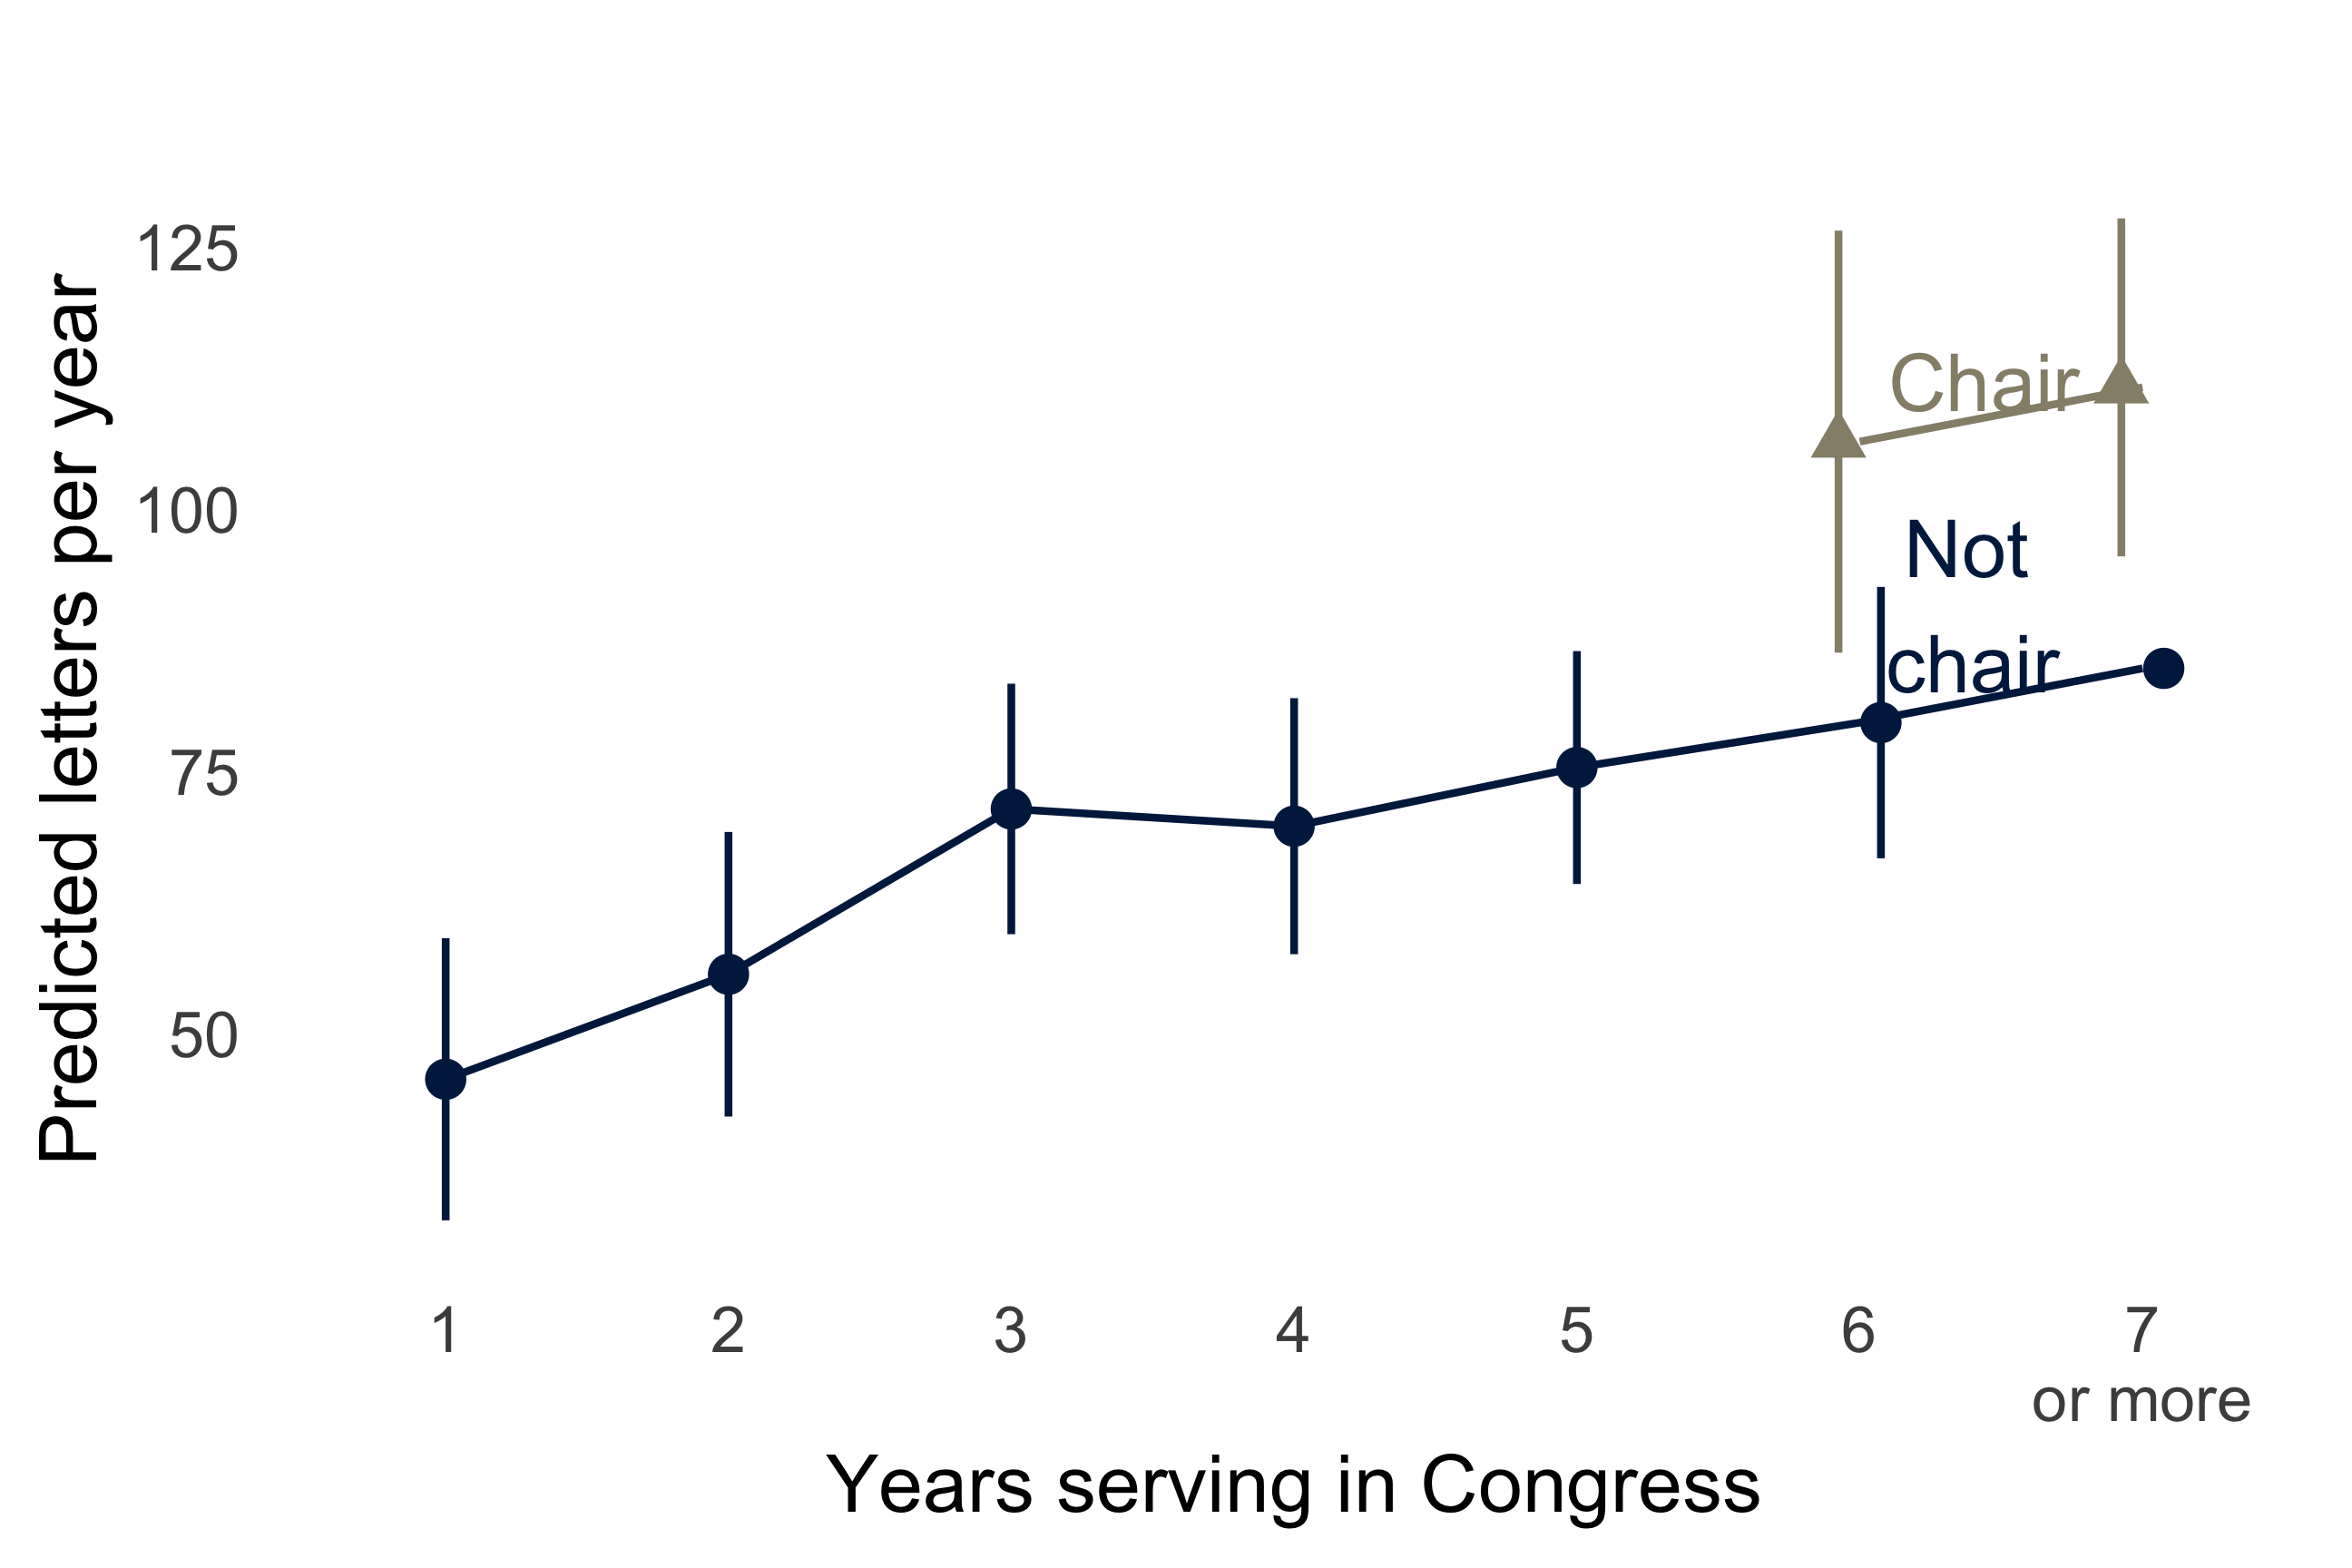
\includegraphics[width = .8\textwidth]{figs/m-total-predicted-4}
\end{figure}

Figure \ref{f:m-total-predicted-time} shows the predicted total number of letters in Congress and committee chair status (comparing predictions for counterfactuals where the same legislator did and did not receive a chairmanship in their sixth year).\footnote{Predictions are based on a legislator-agency pair where (1) the legislators' average annual contacts equaled the overall average, (2) the legislators' number of contacts with the agency equal the average received by that agency, (3) and the agency received an average number of letters.} 

If we interpret this atertaive measure of expierndce as identified, it shows further suppoert for the conclusions of the within-distirct models. In their first year, legislators make significantly fewer requests to agencies than they do in the following year. Subsequent increases are less significant.  


\subsection{Constituency Service Only}

\begin{table}[hbt!]
\caption{The Effect Expierence and Institutional Power on Constituency Service} \label{t:models_con}
\begin{minipage}{\textwidth}
\begin{center}
\begin{tabular}[t]{lcccc}
\toprule
  & (1) & (2) & (3) & (4)\\
\midrule
\textbf{Dependent Variable} & \textbf{Count} & \textbf{Count} & \textbf{Count} & \textbf{Log(Count+1)}\\
\midrule
Committee Chair & \num{0.302} & \num{0.040} & \num{0.044} & \num{0.012}\\
 & (\num{0.108}) & (\num{0.064}) & (\num{0.064}) & (\num{0.007})\\
Ranking Member & \num{0.503} & \num{0.054} & \num{0.070} & \num{0.012}\\
 & (\num{0.108}) & (\num{0.067}) & (\num{0.067}) & (\num{0.007})\\
Prestige Committee & \num{0.321} & \num{0.031} & \num{0.025} & \num{0.013}\\
 & (\num{0.049}) & (\num{0.036}) & (\num{0.036}) & (\num{0.007})\\
First Year & \num{-0.138} & \num{-0.276} & \num{-0.265} & \num{-0.059}\\
 & (\num{0.040}) & (\num{0.055}) & (\num{0.054}) & (\num{0.008})\\
Second Year & \num{0.009} & \num{-0.128} & \num{-0.142} & \num{-0.019}\\
 & (\num{0.046}) & (\num{0.053}) & (\num{0.052}) & (\num{0.008})\\
Third Year & \num{0.030} & \num{-0.070} & \num{-0.088} & \num{-0.011}\\
 & (\num{0.047}) & (\num{0.047}) & (\num{0.046}) & (\num{0.007})\\
Fourth Year & \num{0.061} & \num{-0.055} & \num{-0.072} & \num{-0.006}\\
 & (\num{0.052}) & (\num{0.046}) & (\num{0.045}) & (\num{0.006})\\
Fifth Year & \num{0.001} & \num{-0.069} & \num{-0.064} & \num{-0.011}\\
 & (\num{0.044}) & (\num{0.034}) & (\num{0.033}) & (\num{0.005})\\
Sixth Year & \num{0.070} & \num{0.008} & \num{0.018} & \num{-0.004}\\
 & (\num{0.056}) & (\num{0.044}) & (\num{0.043}) & (\num{0.005})\\
\midrule
Majority & \checkmark & \checkmark & \checkmark & \checkmark\\
Presidents` Party & \checkmark & \checkmark & \checkmark & \checkmark\\
All Legislators & \checkmark & \checkmark &  & \checkmark\\
Served At Least 2nd Term &  &  & \checkmark & \\
Observations & \num{412111} & \num{412111} & \num{388997} & \num{412111}\\
Year x Agency FE & \checkmark & \checkmark & \checkmark & \checkmark\\
Legislator x Agency FE &  & \checkmark & \checkmark & \checkmark\\
\bottomrule
\multicolumn{5}{l}{\rule{0pt}{1em}\footnotesize Robust standard errors in parentheses, clustered by legislator.}\\
\end{tabular}
 % this one is from replication.rmd
\end{center}
\footnotetext{This table shows how the number of contacts hand-coded as constituecy service changes as legislators acquire more expiernece and power in Congress. Column 1 shows the average differences across committee assignments and years in Congress. Column 2 presents the difference-in-differences estimates. Column 3 subsets to legislators who serve at least 3 years in Congress. Column 4 takes the Log of the counts + 1 as the dependent variable.}
\end{minipage}
\end{table}

Table \ref{t:models_con} is identical to Table \ref{t:models_total} except that we subset the data to only legislator requests hand-coded as constituency service. 
Model 2 (Column 2 of Table \ref{t:models_con} and Figure \ref{f:m-con-predicted}) provide the estimated effects from the difference-in-differences specification in Equation \ref{e:diff1}. More experience increases the level of constituency service that legislators provide. The effect of being a committee chair is positive but not significant at the .05 level. We estimate that the experience gained between the first and second year in Congress causes an increase of 0.15 requests \textit{per agency}. The experience gained between the first and seventh years causes an increase of 0.28 per agency. Across all 90 agencies, this represents an increase of approximately 25 additional requests per year, 38.6\% of the average number of requests per year in our data. There is a smaller increase after the second year. The experience gained between the second and seventh year causes an increase of 0.13 per agency, an increase of approximately 12 additional requests per year, 38.6\% of the average number of requests per year in our data.


\begin{figure}[hbt!]
\centering
\caption{Predicted Number of Constituency Service Requests} \label{f:m-con-predicted}
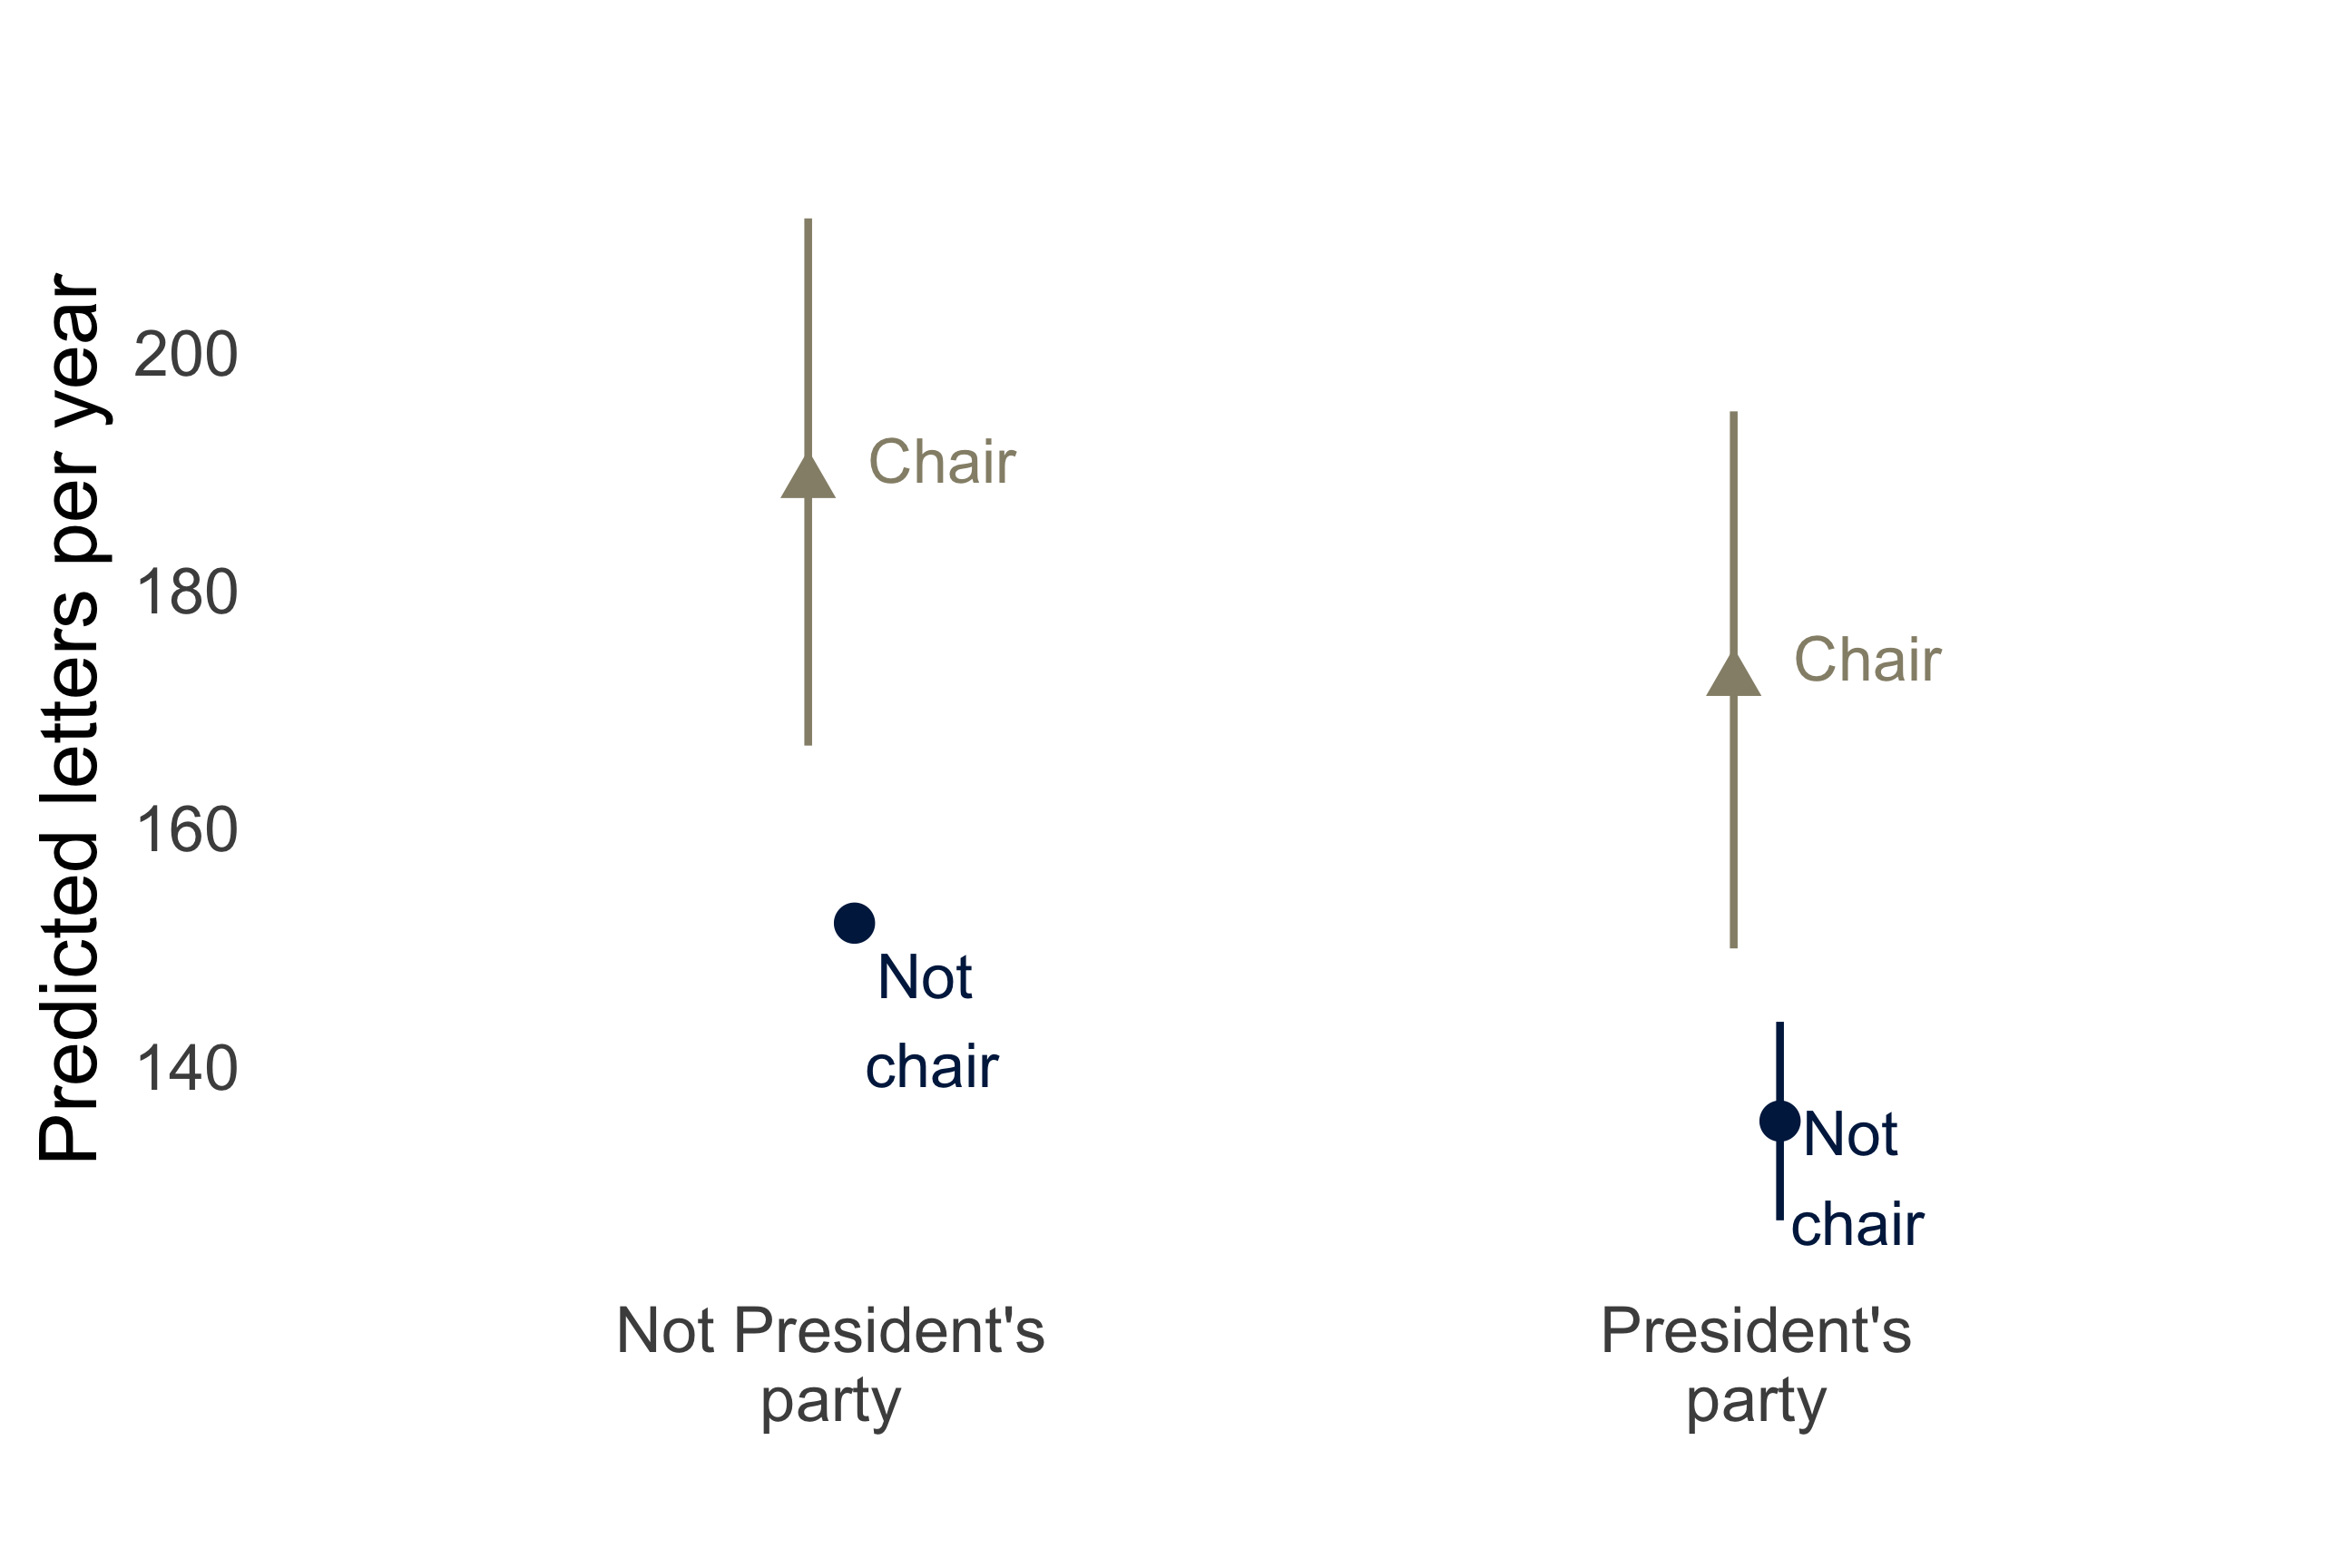
\includegraphics[width = .49\textwidth]{figs/m-con-predicted-1}
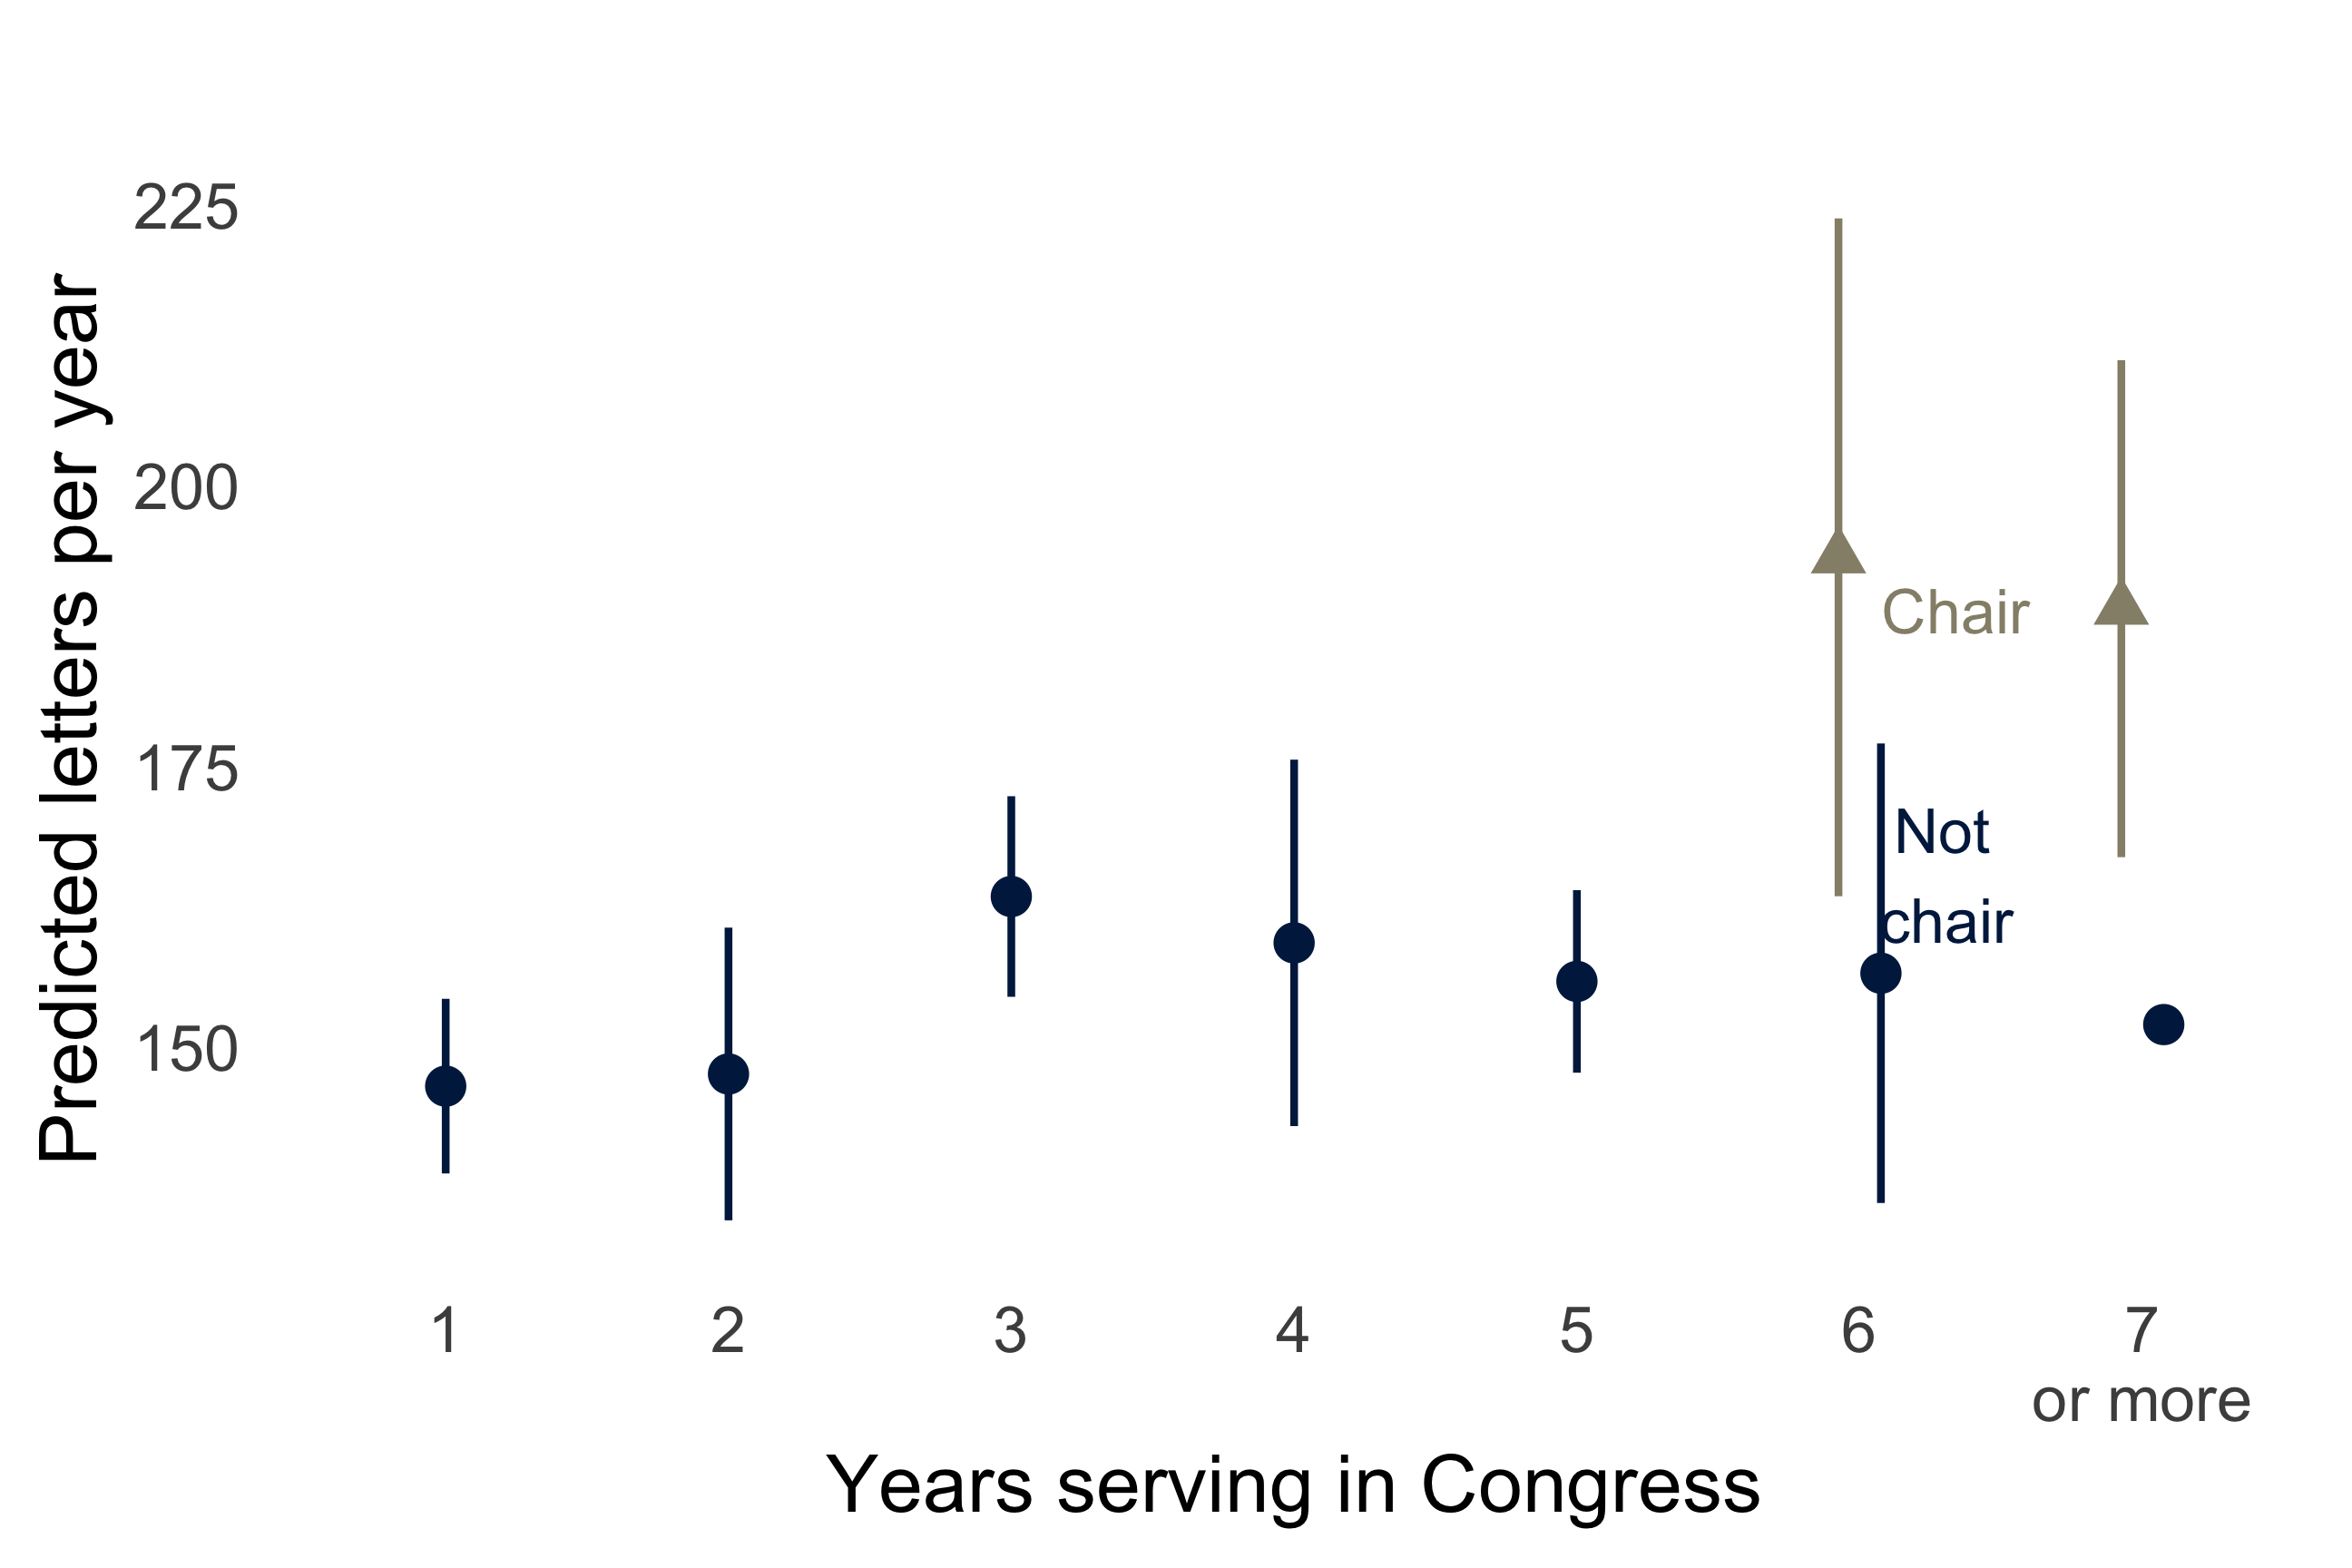
\includegraphics[width = .49\textwidth]{figs/m-con-predicted-2}
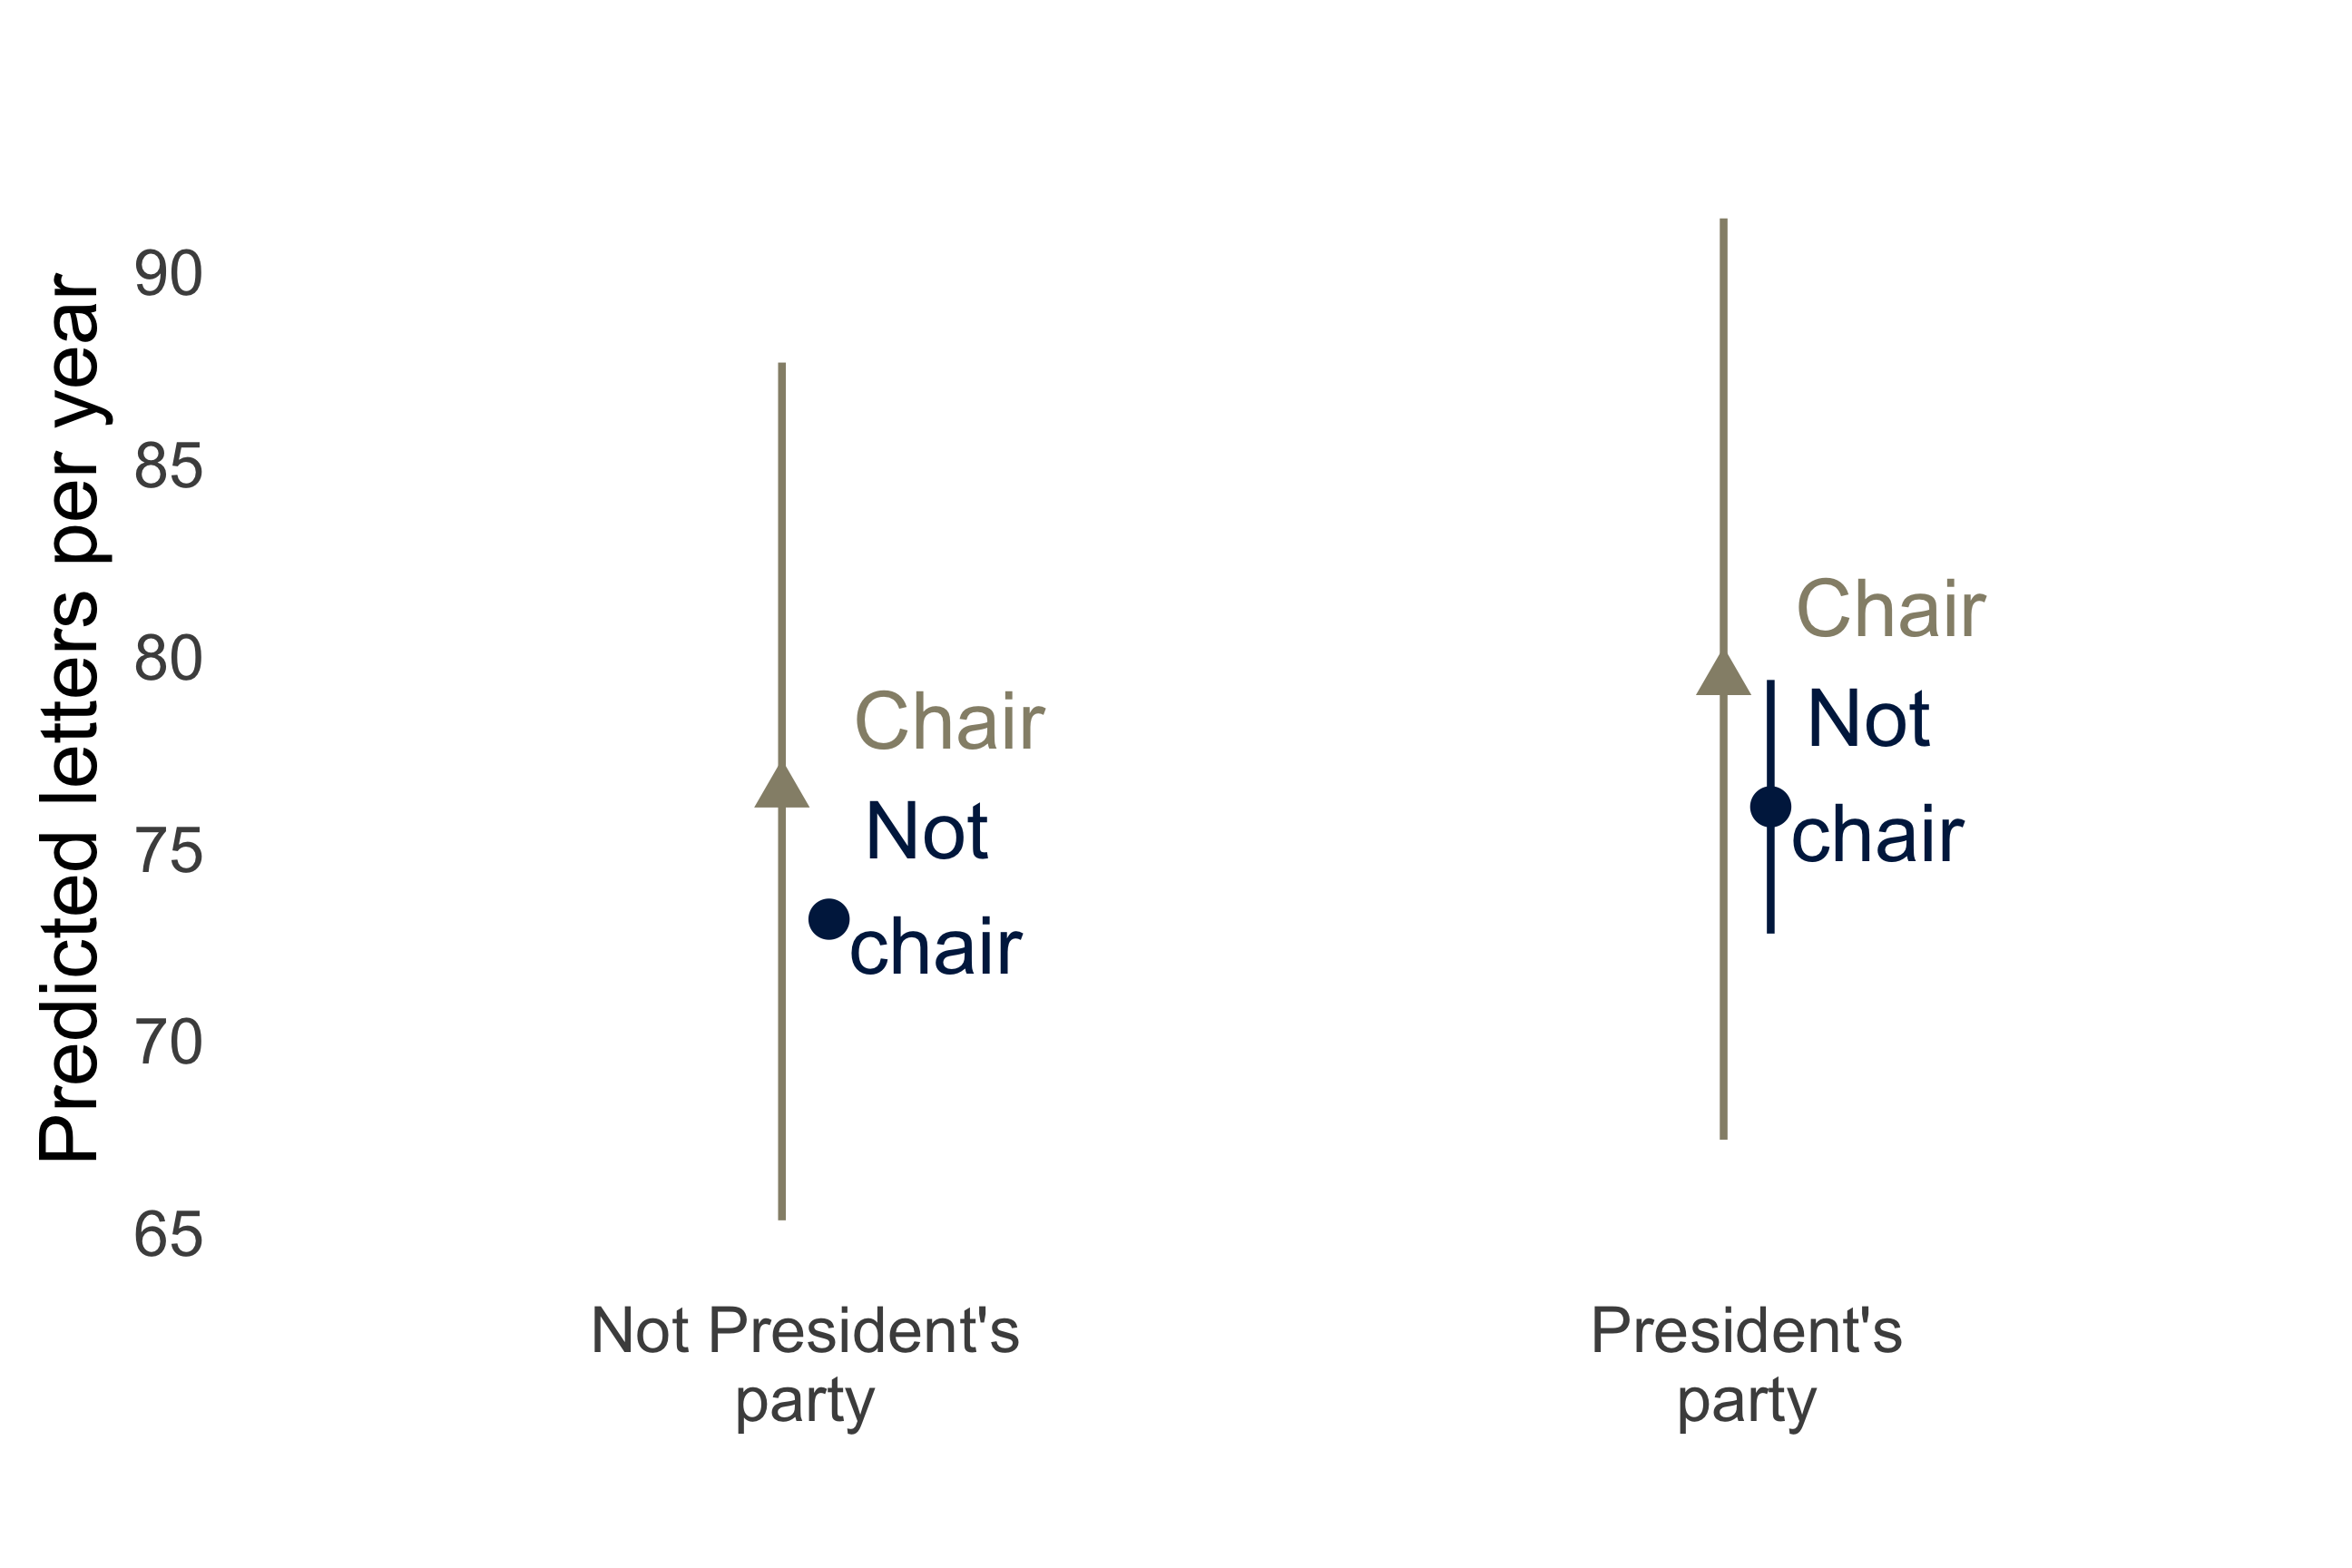
\includegraphics[width = .49\textwidth]{figs/m-con-predicted-3}
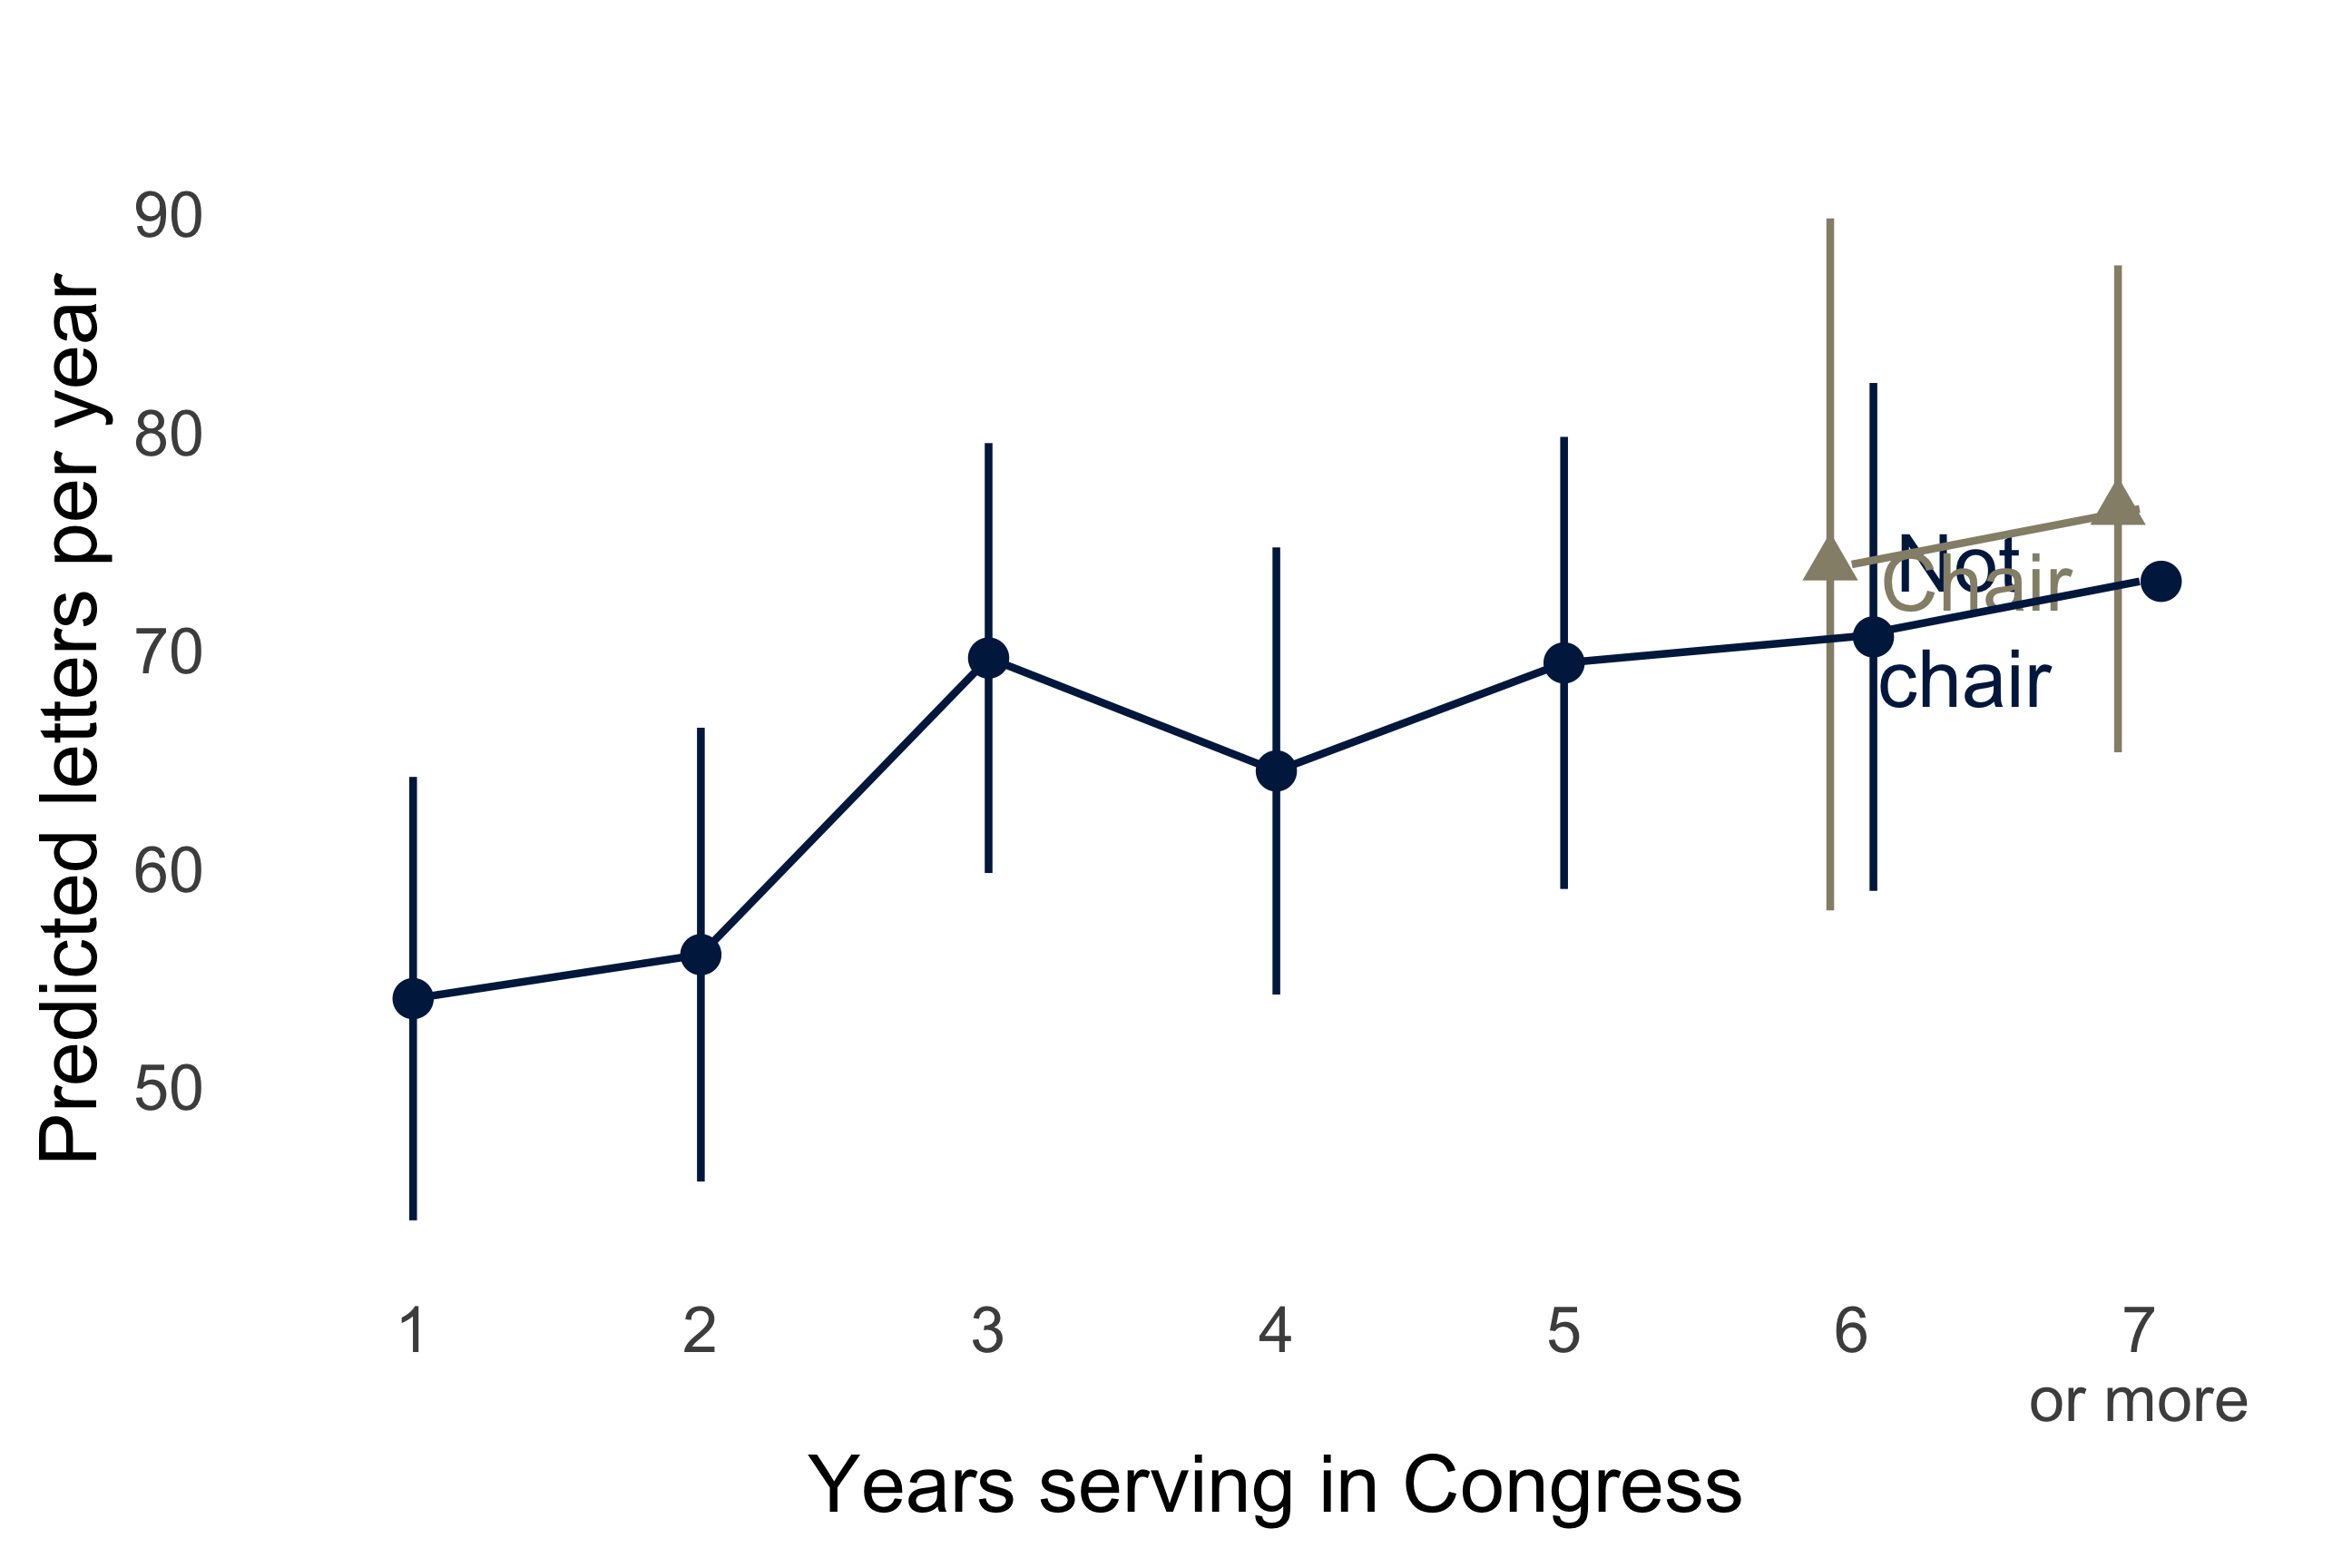
\includegraphics[width = .49\textwidth]{figs/m-con-predicted-4}

\end{figure}

\subsection{Policy Work Only}

\begin{table}[hbt!]
\caption{The Effect Expierence and Institutional Power on Policy Work} \label{t:models_policy}
\begin{minipage}{\textwidth}
\begin{center}
\begin{tabular}[t]{lcccc}
\toprule
  & (1) & (2) & (3) & (4)\\
\midrule
\textbf{Dependent Variable} & \textbf{Count} & \textbf{Count} & \textbf{Count} & \textbf{Log(Count+1)}\\
\midrule
Committee Chair & \num{0.199} & \num{0.158} & \num{0.159} & \num{0.036}\\
 & (\num{0.027}) & (\num{0.034}) & (\num{0.034}) & (\num{0.007})\\
Ranking Member & \num{0.145} & \num{0.090} & \num{0.092} & \num{0.025}\\
 & (\num{0.028}) & (\num{0.024}) & (\num{0.024}) & (\num{0.005})\\
Prestige Committee & \num{0.049} & \num{0.031} & \num{0.031} & \num{0.010}\\
 & (\num{0.009}) & (\num{0.010}) & (\num{0.010}) & (\num{0.003})\\
First Year & \num{-0.076} & \num{-0.076} & \num{-0.070} & \num{-0.030}\\
 & (\num{0.007}) & (\num{0.016}) & (\num{0.016}) & \vphantom{1} (\num{0.004})\\
Second Year & \num{-0.045} & \num{-0.042} & \num{-0.040} & \num{-0.018}\\
 & (\num{0.007}) & (\num{0.016}) & (\num{0.016}) & (\num{0.004})\\
Third Year & \num{-0.042} & \num{-0.031} & \num{-0.033} & \num{-0.013}\\
 & (\num{0.008}) & (\num{0.013}) & (\num{0.013}) & (\num{0.004})\\
Fourth Year & \num{-0.021} & \num{-0.011} & \num{-0.013} & \num{-0.006}\\
 & (\num{0.009}) & (\num{0.013}) & (\num{0.013}) & (\num{0.004})\\
Fifth Year & \num{-0.022} & \num{-0.009} & \num{-0.011} & \num{-0.006}\\
 & (\num{0.009}) & (\num{0.011}) & (\num{0.011}) & (\num{0.003})\\
Sixth Year & \num{-0.011} & \num{0.002} & \num{0.003} & \num{-0.006}\\
 & (\num{0.012}) & (\num{0.012}) & (\num{0.012}) & (\num{0.003})\\
\midrule
Majority & \checkmark & \checkmark & \checkmark & \checkmark\\
President's Party & \checkmark & \checkmark & \checkmark & \checkmark\\
All Legislators & \checkmark & \checkmark &  & \checkmark\\
Served At Least 2nd Term &  &  & \checkmark & \\
Observations & \num{412111} & \num{412111} & \num{388997} & \num{412111}\\
Year x Agency FE & \checkmark & \checkmark & \checkmark & \checkmark\\
Legislator x Agency FE &  & \checkmark & \checkmark & \checkmark\\
\bottomrule
\multicolumn{5}{l}{\rule{0pt}{1em}\footnotesize Robust standard errors in parentheses, clustered by legislator.}\\
\end{tabular}
 % this one is from replication.rmd
\end{center}
\footnotetext{This table shows how the number of hand-coded policy work contacts changes as legislators acquire more expiernece and power in Congress. Column 1 shows the average differences across committee assignments and years in Congress. Column 2 presents the difference-in-differences estimates. Column 3 subsets to legislators who serve at least 3 years in Congress. Column 4 takes the Log of the counts + 1 as the dependent variable.}
\end{minipage}
\end{table}


Table \ref{t:models_policy} is identical to Table \ref{t:models_total} except that we subset the data to only legislator requests hand-coded as policy work. 
Column 2 of Table \ref{t:models_policy} and Figure \ref{f:m-policy-predicted}) provide the estimated effects from the difference-in-differences specification in Equation \ref{e:diff1}. Across all measures of institutional power, we find that more power increases the level of policy work that legislators provide. Consider first the effect of being a committee chair. We estimate that becoming a committee chair causes an increase of 0.16 policy requests \textit{per agency} (95-percent confidence interval [0.09, 0.22]). Across all 90 agencies, this represents an increase of approximately 14 additional requests per year, 92.6\% of the average number of requests per year in our data. There is a smaller increase for individuals who become ranking members and those who join a Prestige Committee, though the increase is statistically significant for the prestige committee. Becoming a ranking member of a committee causes an increase of 0.09 contacts per agency while joining a prestige committee causes a 0.16 per agency increase in the number of contacts a member of Congress makes.

\begin{figure}[hbt!]
\centering
\caption{Predicted Number of Policy Requests} \label{f:m-policy-predicted}
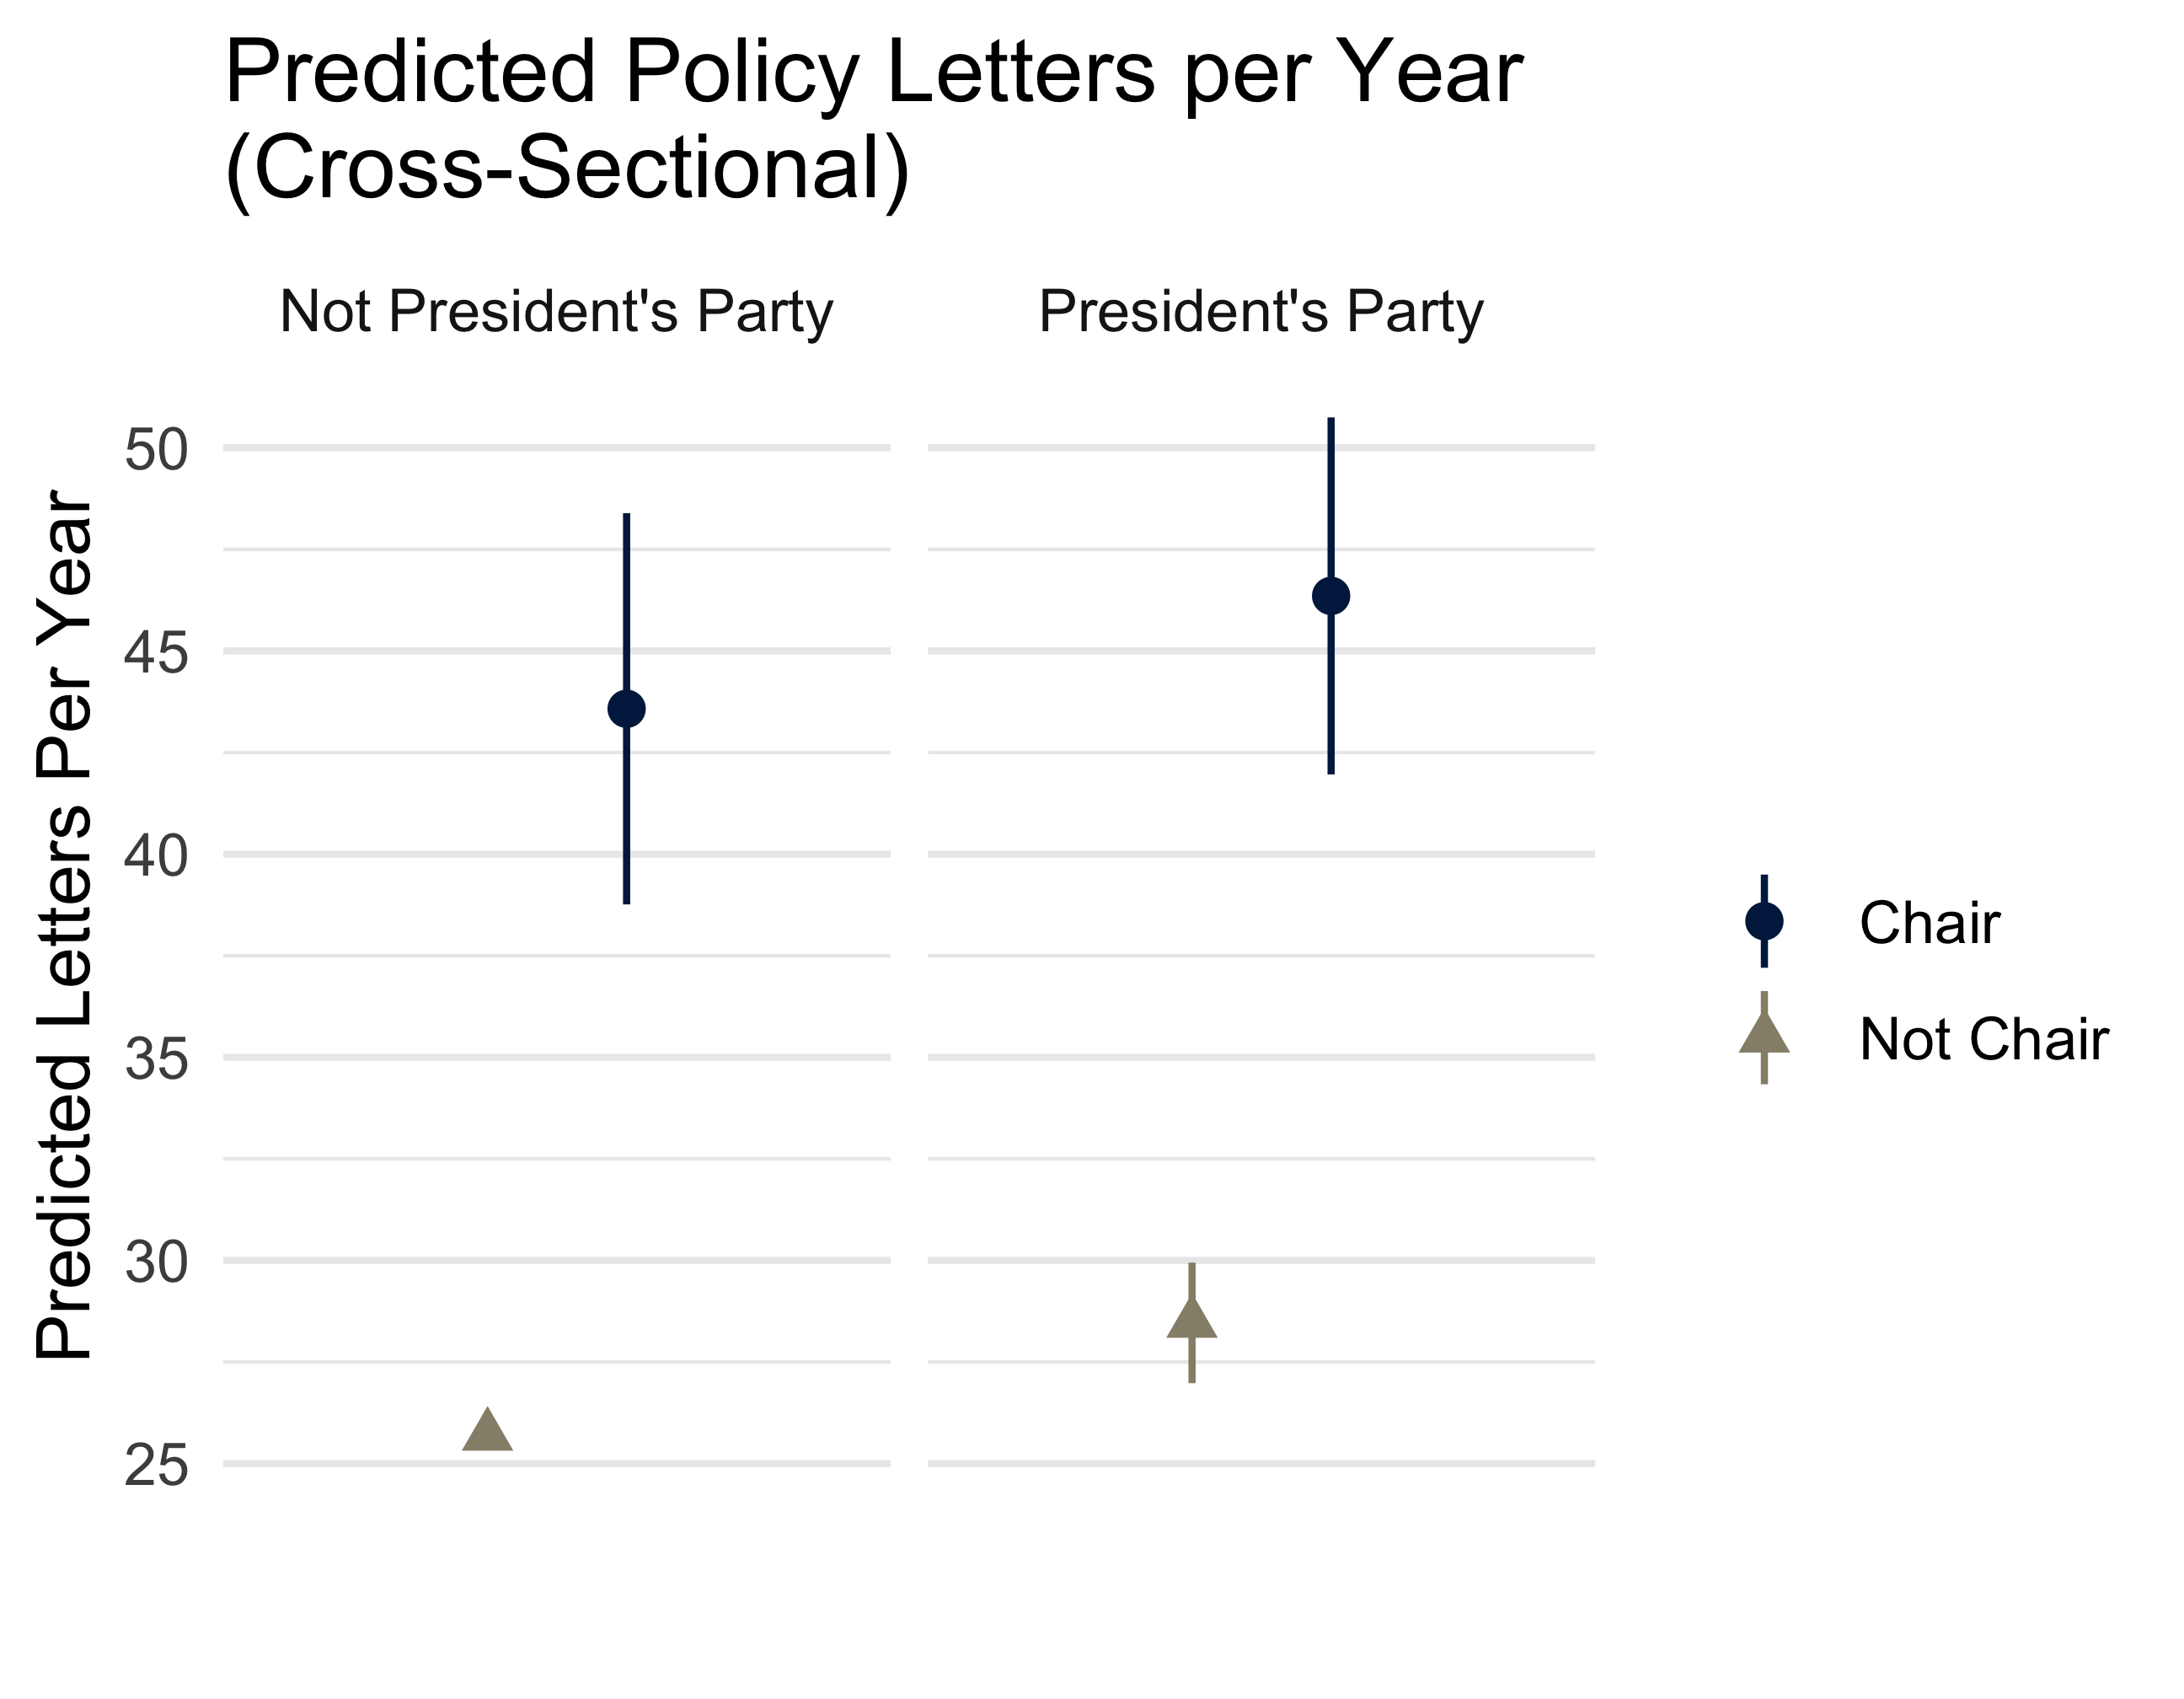
\includegraphics[width = .48\textwidth]{figs/m-policy-predicted-1} 
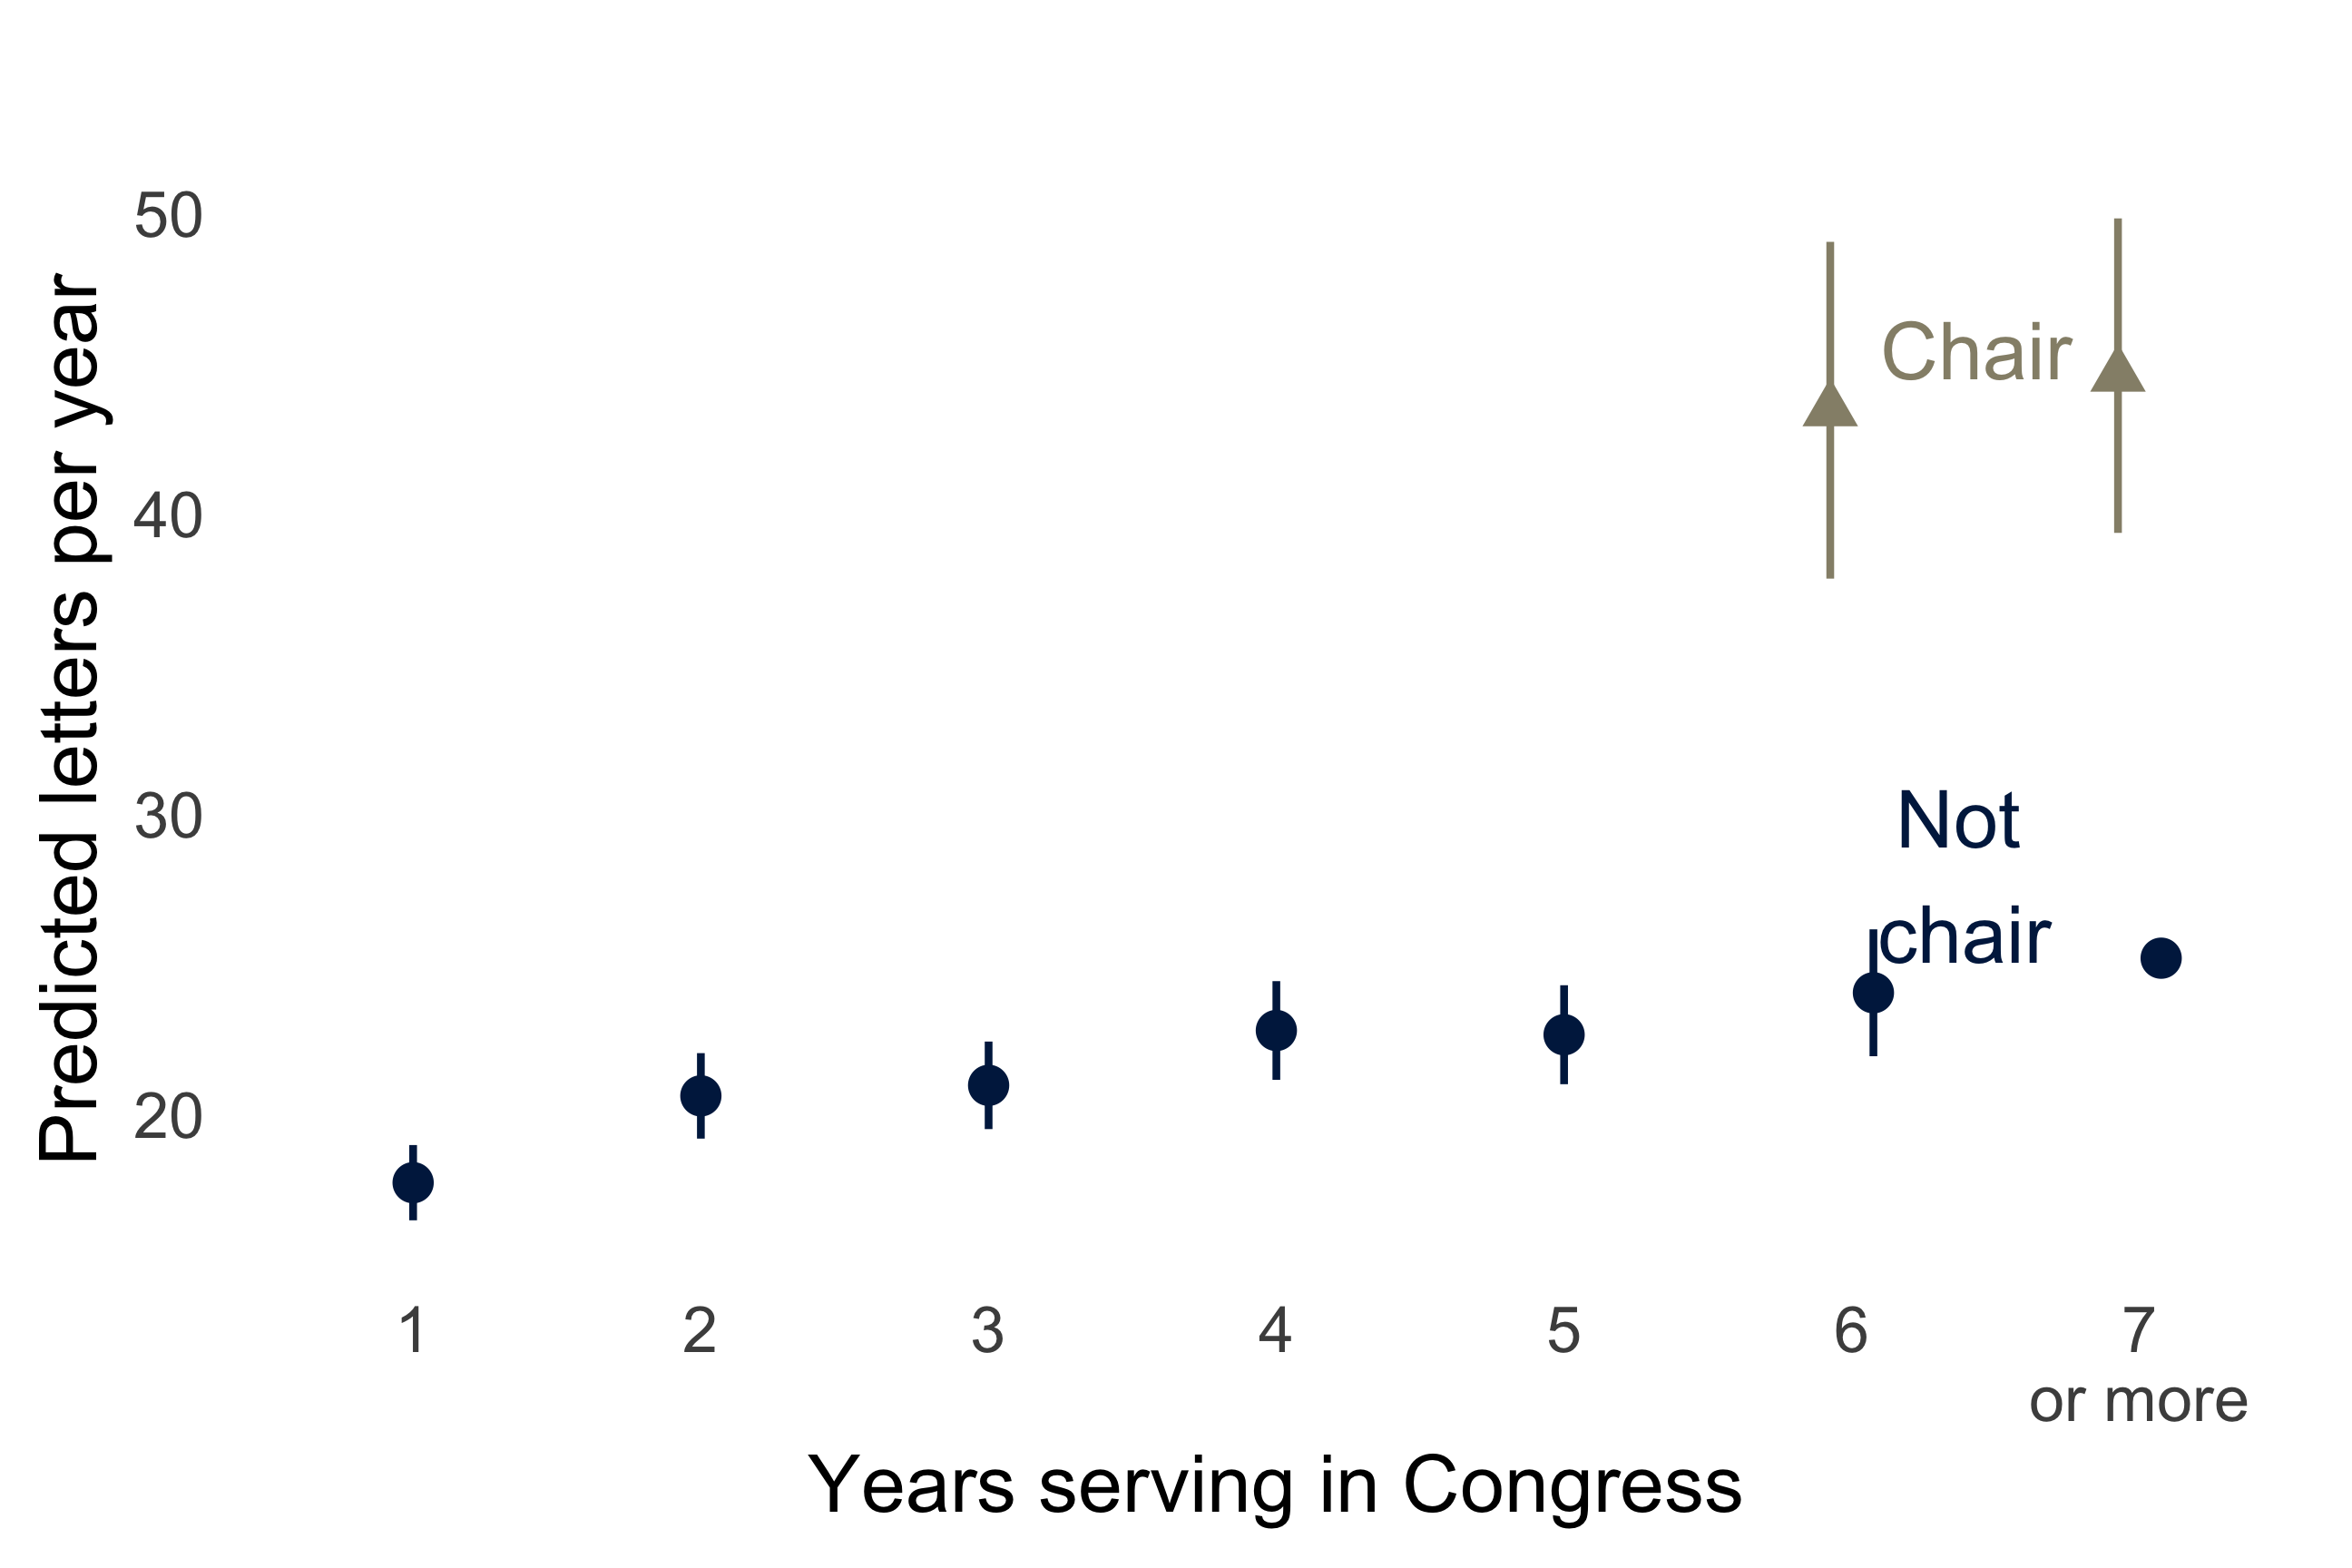
\includegraphics[width = .48\textwidth]{figs/m-policy-predicted-2} 
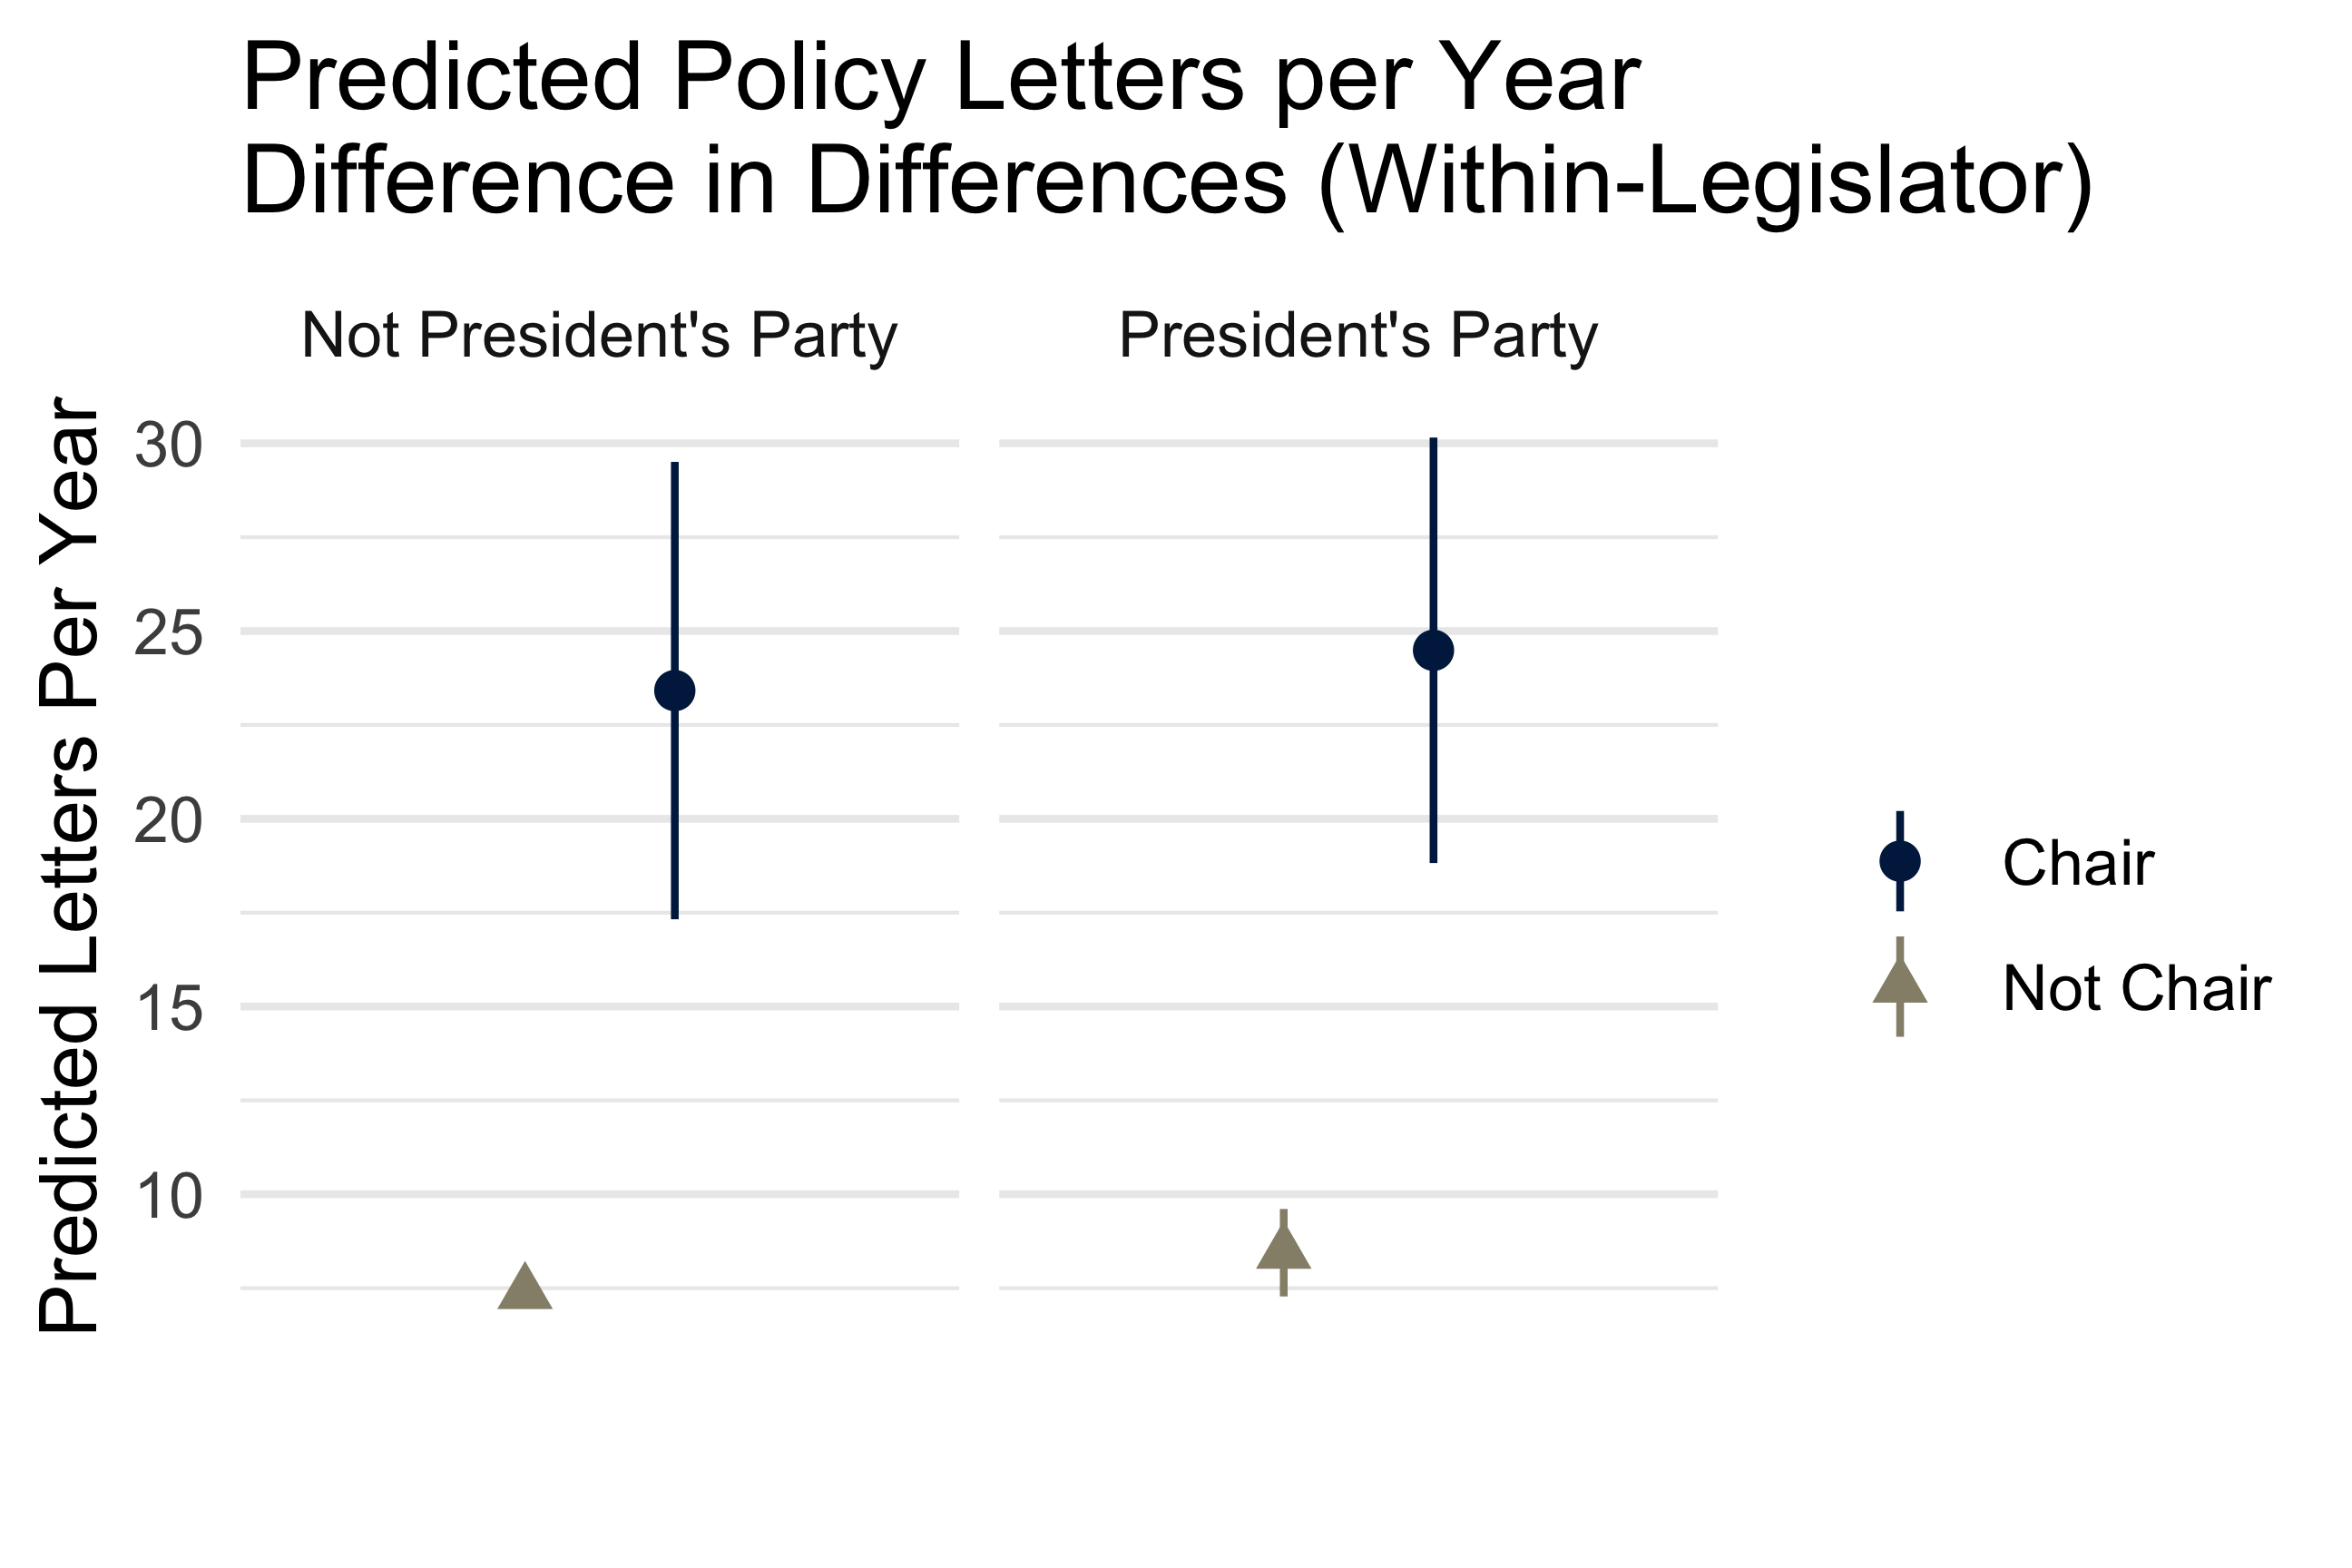
\includegraphics[width = .48\textwidth]{figs/m-policy-predicted-3} 
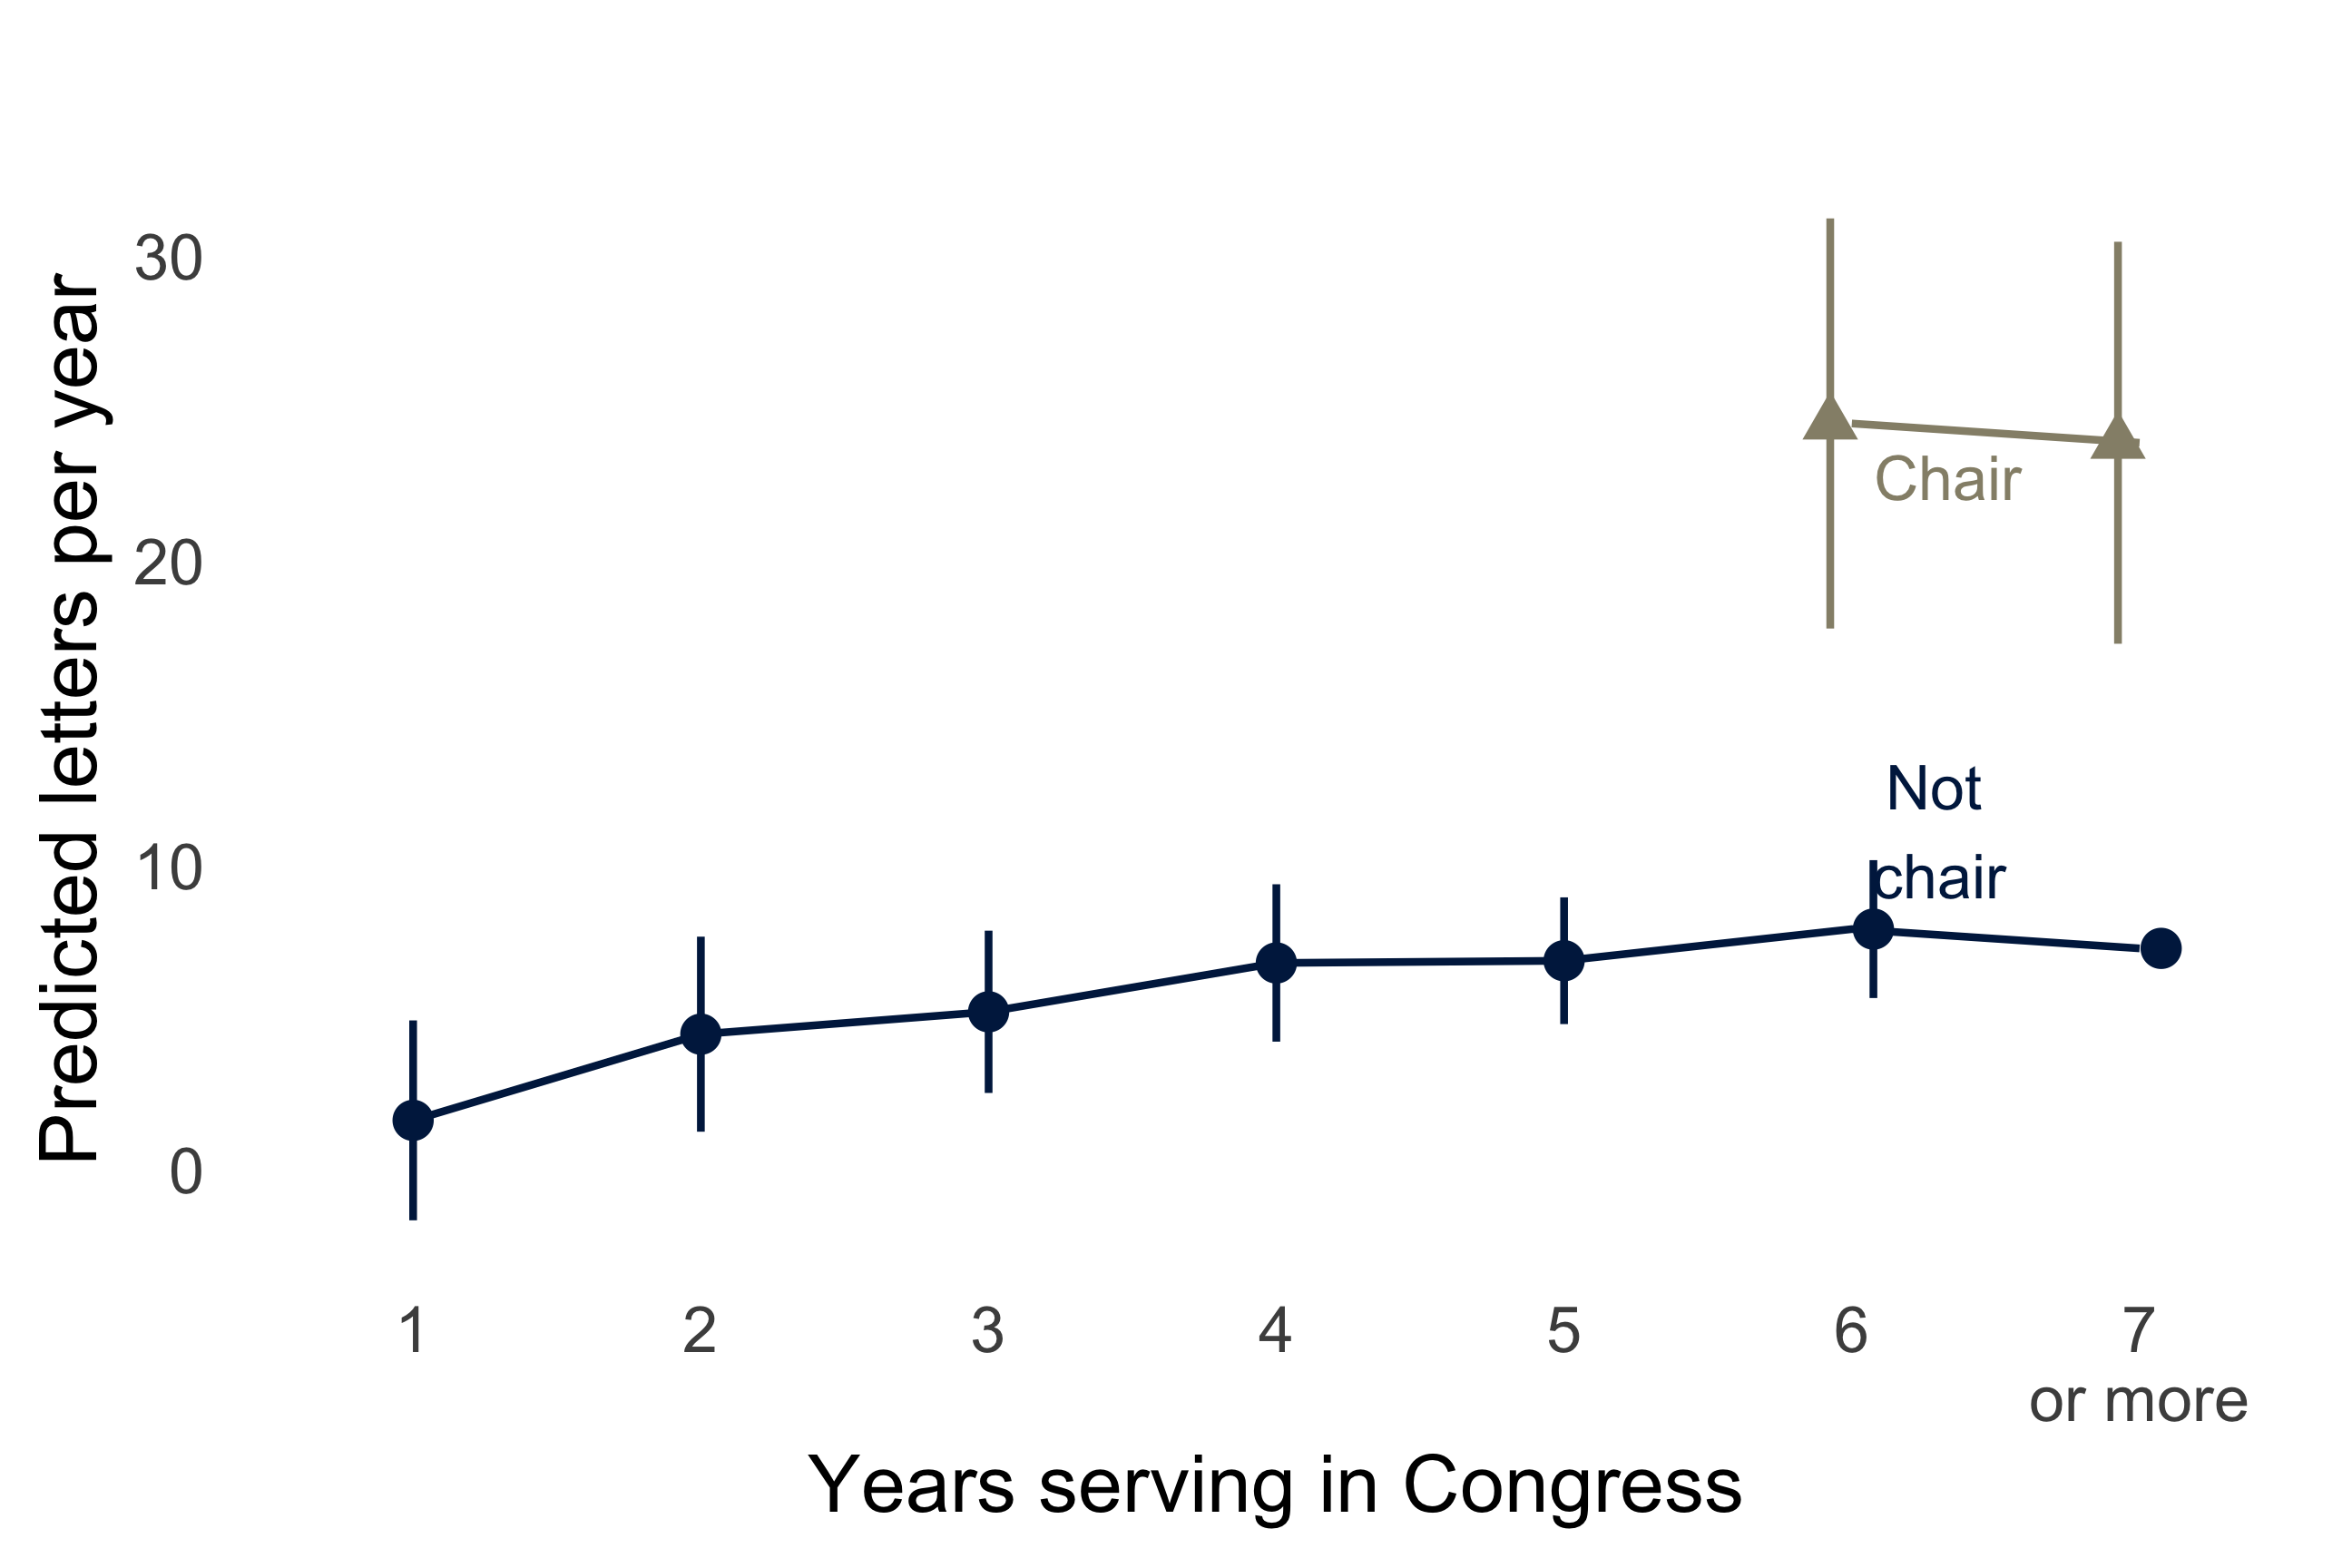
\includegraphics[width = .48\textwidth]{figs/m-policy-predicted-4} 

\end{figure}


